\documentclass{book}

\usepackage[backend=biber]{biblatex}
\bibliography{uni.bib}
\usepackage{csquotes}
\usepackage{fancyhdr}
\usepackage{multicol}

\pagestyle{fancy}
\fancyhf{}
\fancyhead[LE,RO]{Kyle Eggleston}
\fancyhead[RE,LO]{Living :: A Journey}
\fancyfoot[CE,CO]{\leftmark}
\fancyfoot[LE,RO]{\thepage}
\renewcommand{\headrulewidth}{2pt}
\renewcommand{\footrulewidth}{1pt}

\title{%
  Living \\
  \large A Journey}
\author{Kyle Eggleston}
\date{Jun 3, 2018 - Dec 31, 2018}

\begin{document}
\maketitle
\thispagestyle{empty}

\frontmatter

\section*{Introduction}

Ah what is a life that cannot be lived? Who is to say it will come and go as you
please? No one has the ability to say such things. It is but a falst narrative
from which you can easily fall down a shaft and die. Did not the poet say:

\begin{displayquote}
Prick us do we not bleed.\footnote{Shakespeare - The Merchant of Venice}
\end{displayquote}

Yes, that is what happens in life when you haven't the faintest idea of where
you are headed. Perhaps it is more easily meant if one were to understand that
which we cannot easily see for we look through a mirror 
darkly.\footnote{1 Corinthians 13:12}

To say that we have the full truth, as it were, is to feign ignorance on 
whatever there is other people are able to bring to us as a whole. We are not to 
push them away but embrace them, accept them and what they have to bring to the
table. yet we get caught up in our own ways that we do not know where to begin
and where to end. We are at a loss in this time in life, and it is a pity.

Not everyone wants to believe in the same ideals as you do. Not everyone wants
to have the same thoughts as you do. Not everyone is the same. Yes we can be 
\textit{one} as it were, but not everyone comes from the same background. We 
are all different in our own ways. Should that alone not be celebrated?
Diversity in numbers and types of people? Different cultures and backgrounds? We
can each learn something from one another.

\mainmatter

\chapter{Journal Entries}
\section{Sun, Jun 3, 2018}

Oh what a day today has been. It is but a Sunday. I do not feel any different
now then I ever did on a Sunday. Perhaps my mind doesn't know how to accept that
which it cannot accept? I do not know the meaning of such language, however here
I am and that is all which matters. I'm sure the church people will get ahold of
me eventually. But it is of no concern to me.

I do what I do, and I try what I try. There is no reason for any of this
nonsense to follow me. If it does follow me? Then it will follow me. Again, I
see no reason for it to have any kind of impact on my life.

Now if you were to ask my parents about such things, they would tell you I am a
child of hell and will be going there after this life is over. That may be the
case, but if what I've learned about heaven is true I'd rather not go there to
begin with. Whatever the case this life will continue to be whatever it will be
and there is nothing wrong with that to me.
\section{Mon, Jun 4, 2018}

Today is like any other day. There is nothing going on that I cannot see myself
doing. It is a unique challenge of a day. Kids are out of school, good for them.
However, I long for those days where I had a summer break from life. Being a kid
was amazing. Yes, there were rules to live by etc. but that didn't make life any
less worth it. I often find myself wondering why I wanted to grow up so quickly.
There was no need for it...was there? I didn't think there would be much of a
need. Either way, this life did what it does best and it took me and chopped me
down to nothing. So here I sit. Waiting for whatever is to come my way.

You would think this life would be easier by now. I've been alive for how many
years and I still don't have the slightest clue of what on earth I'm doing.
Literally. What is my whole purpose here? I do not know. Should I have a clue of
what I am doing here? That would be nice...but I simply do not have a clue.

Does it matter in the grand scheme of things? I'm not a fan of that term though.
``Grand Scheme." What exactly does it mean? I do not know. It's probably just a
phrase that doesn't make sense or matter. Such a silly life and thing to worry
about, yet here I am worrying about it. What on earth is that even about? No
clue. Perhaps it doesn't matter at all? That would be nice.

I feel like I'm rambling\footnote{To talk or write at length in a confused or 
inconsequential way.} now. Good bot, you'll do fine.

Where was I? Oh yes, the purpose of why I am here. They say time is an enemy. It
finds its prey and will destroy you eventually. That is not a lie. Time is quite
an evil enemy, why wouldn't it want to destroy you long before you are able to
grasp onto what is going on?

There are days where I wish time wasn't such a blatant barrier in my way. It
would be nice to be able to look around and understand or grasp that which I
need to.\footnote{It should be pointed out, I never know what I'm talking about. 
You might wish to skip this portion of thought. To say I have a complete 
understanding or grasp of what I am doing? No, it's a nice thought but no. I 
mean, there could be various thoughts and practices ahead of a person. They 
simply do not understand or know or grasp all that is meant to be taken in
at a given moment in time. Is it not better for a person to grasp something 
fully before they are to be taken into that which is considered the unknown?}

But here I am, living a life that was meant to be something. It did mean 
something one day, one frame of measurement in life. It had a meaning. Now? 
Not so much. Oh well, time will figure itself out eventually. There is no reason
for it not to.

There is an excellent quote I heard once regarding censorship:

\begin{displayquote}
With the first link, the chain is forged. The first speech censured, the first 
thought forbidden, the first freedom denied, chains us all 
irrevocably.\footnote{Star Trek: The Next Generation - The Drumhead}
\end{displayquote}

Censorship can be the worst frame of mind to impose on any given society or
individual. It indeed does cause harm and has the ability to destroy a
civilization. I wonder why society, religion, other beliefs put censorship at
the top of their game. Maybe it's a form of control over a person or group? If
such control that disallows independant thought occurs, then I'm guessing not
many people would want to be part of that group whatsoever. But that's just my
thought on the matter. I know I wouldn't want to have anything to do with it. I
would rather die than to be locked away without the ability to voice my opinion
on a matter or my thoughts. Talk about a nightmare.\footnote{A terrifying or 
very unpleasant experience or prospect.}

So here we are. What's left of humanity. In the not too distant future, people
will become slaves of their own technologies. It is already beginning to happen
today. You can't walk down the street without seeing someone on their phone. It
is but a waste of time for some, others it is their life. Whatever they do and
say, they have to have their phone with them. They cannot live without that form
of tech. It's a shame really. A shame that people cannot live in this day and
age without holding onto a simple device.

But to each his own as the phrase goes.\footnote{I'm not even certain who came
up with that phrase. Seriously. Who would coin such a phrase? We should google
it. Hold please...google tells me it's been around since the 1500s, but the 
modern wording was first recorded in 1713. Thank you Google and thank you
dictionary.com for those spleneded pieces of history. Yeah something like that.
Either way? It's a phrase that can mean a great deal of whatever for whoever
when it comes about. Whatever the case, life continues onward.} As people grow
so does technology. No one is exempt from any of it. This life will continue
to propser and grow as it always does. There's nothing wrong with that. Life
has a way to do many marvelous things. There isn't a reason why it shouldn't be
able to continue with such knowledge.

I am not one to condem such practice as it were. There's no reason a person
cannot live in the here and now. I just find it sad that they cannot put their
phone down to pay attention to the important things going on in life. Such a
dismal state of affairs which we live.

Naturally there will be those who would want you to believe in all freedoms.
That is fine. But when your freedom interferes with your work, or your family
duties? There needs to be an end to such a freedom. Yes you can dabble in this
that and the other, but do not allow it to overrun your life. That's not the
purpose for such tools and devices.
\section{Tue, Jun 5, 2018}

Life is difficult at times. Today is one of those days where it is extremely
hard. I don't want to talk about it, but I need to talk about it. Yes it's one
of those days indeed.

Money is always an issue when it comes to life. I wish we didn't have to deal
with money problems. That would be great. A better alternative to it? I do not
have the faintest idea of what that could be. But something different would be
amazing right now.

But we have to deal with money. It's really a root of evil in my opinion.
Whatever happens happens though. I just hope it will happen sooner rather than
later.
\section{Wed, Jun 6, 2018}

Oh hello brand new day! How are you doing today? There isn't much of a thing to
think about. How nice would that be? Yes, it would be very nice. But it's not.
Life isn't nice that way.

Things should be going good. There is a lot of things that don't go well in
life, life itself shouldn't be one of them. At least to my thinking that's how
none of it should happen. Life needs to be better. It needs to find a way to
become easier? Maybe that's not the right word for it. I don't know what word to
use actually. Easier life...doesn't always make sense.\footnote{Whoever said
this life was easy sure didn't understand what they were getting into.} So we
live a life that's full of confusion and complaint...and whatever else there is
to deal with. This life doesn't always make sense. This life will never make
sense. We have to roll with the punches as it were.\footnote{``Roll with the
punches"??? Where the hell did that phrase even come from? It's not a phrase
that makes much sense! Seriously, who ``rolls" with anything these days? Either
you get with the program or you get smacked down. Isn't it that simple?}

Let's not dwell on the past. The past can only conjure up problems and issues.
To focus soely on the past is to focus on things which will only bring
heartache. A heartache so deep, you don't have a clue where you will end up. It
hurts to be that way. Hurts to not understand anything that's going on. Life
isn't full of wisdom. Life is full of hurt. There is no happiness around this
life, either you walk a certain path, one of your choosing, or you fail.

Failing doesn't always mean certain death. No, not at all. To fail is but a part
of human existence. Everyone fails in their life from time to time. There's
nothing wrong with that. Just remember that when you do fail, to stand back up
and get on with your life again. To fail is not a final resting place, it is but
a temporary marker as it were. You are able to stand from it. There is no shame
in failing.
\section{Thu, Jun 7, 2018}

Another day is here. There are some days which just don't make sense. I believe
today is one of those days. Why would it make sense? There's no reason for it to
make any sense at all. Yet here we are, trying to make sense of all and
everything which doesn't matter. It's life right? Such a life which doesn't want
to make sense will never make any sense. Yet, we expect it to do something and
have some kind of purpose that has reason to it. It's not a clear and cut dry
solution. That's what this life is all about. Nothing makes 100\% sense all of
the time.\footnote{Imagine for a second, a moment if you will, that life had
the ability to make perfect sense. There would be no confusion about how 
anything is meant to play out. Think about that for a moment. No fear of anyone,
no hatred, no grief, everything in perfect peace. I doubt we'll ever see that
in this life...perhaps in the next life to come. Who's to say exactly how any
of it will work.}

It would be nice for everything to have some kind of order to it. I wonder how
that would be exactly. If everything was in order, there wouldn't be much of a
problem would there? People would get in line. They wouldn't fight each other?
If there is order to a chaotic world, where does that leave the chaos? Where
would such chaos exist or go? Is it possible for an entire civilization, an
entire world to live in complete harmony?

We're told in the Book of Mormon after Christ's visitation to the America's,
there was a long period of peace between the Nephies and the Lamenites, that
there were no manner of ites.\footnote{4th Nephi 1:17} They were all one in 
purpose...finally they had achieved harmony. Eventually it went away, as does 
all kind of harmony as evil crept back in and destroyed civilization after 
civilization. But to have such a peace? How wonderful would that be!

We live in a world where destruction can come at any moment. There's no reason
to necessiarly fear it, but to be aware of such things. We are to be prepared in
all things that might come our way.

Naturally it would be good to find peace and harmony among all people. To not
worry about anything that might be of destruction to us, but life doesn't always
work out that way. It has a tendency to destroy us from within. That is, it can
destroy us from inside of an organization. There is always that one wolf in
sheeps clothing. Someone always has the intent on destroying a structure from 
the inside. Where is the justice in such an action? I cannot say for certain,
but it would appear such things would be bad.
\section{Fri, Jun 8, 2018}

40 Years ago today. The Priesthood and Temple Ban on the Negro race was lifted.

There is in this life truths which cannot be denied. There are times when men
speak for God without asking God if they should say such things. It can be
rather embarrassing later on down the road when they have to change their speak,
claiming it to be from God or that God never instructed them to say such things.

As a body, we are expected to listen to their explaination of it all and simply
accept it. Moving forward as though none of it ever happened. This is not how
life works though. It is not in human nature to simply forget something happened
when in fact it did. There is no denying what was taught.

Yes we can move forward from such an act. But we cannot forget what happened in
order to not repeat the past. I hope that makes some kind of sense. It is better
to move forward into the future without repeating past mistakes than it is to
create those mistakes all oever again.

Naturally it is better to have not made such foolish statements to begin with,
but I fear that is human nature. I would say more on this topic, but I fear I
might get too heated. I do not wish that.\footnote{I of course am speaking about
blacks finally receiving the blessings of the priesthood and the temple after
so many years of prophets and aposltes having anti feelings towards them as a 
race. In my opinion, it should never have happened. They should have always
had the blessings allowed them, because God is not that author of confusion,
and God is not a respector of men.}

\chapter{Religion Articles}
\chapter{Indoctrination}

I never thought I would end up writing something like this. I suppose it was
really inevitable. Truth claims come and go like a dime a dozen and everyday
there are more people seeking the truth and yet they find more questions.
Official authorities don't ever have any answers regarding these truth
questions. So where does that leave us? I suppose it leaves us waiting and
wanting something to believe in that is true. Something to be able to grab hold
of and say ``yes, this is it!"

Instead we are left to that which we cannot tell is truth. It feels like
something that isn't truth. Something so beyond the truth that we simply cannot
reason with it anymore. It is one to drive a person mad.

A little bit about me. I was born in the covenant. That is, my parents were
sealed in the temple when I was born. I grew up in the church  my entire life. I
served a mission, got married in the temple. Kept my nose clean for most of it.
Sure there were bumps in the road as people have. But nothing I didn't overcome
through the proper channels.

I first ran into what is known as ``anti" material while on my mission. An
investigator had some pamplets. We explained it was incorrect information and
tossed it in the trash without even looking at it. Hey, we were there doing the
Lord's work right? So yeah, it felt like the right thing to do. Toss it away
don't look back.

Oh how I would love to go back in time to that moment. I would have read through
it. Looked it over and saw what there was to see. But I was playing the good
role of missionary. There was no reason for me not to. Little did I know I would
end up with the knowledge that I have years later. What a fool I had been.

I have never felt comfortable with the church. I don't know if it's just because
I didn't enjoy going to church as a kid? I don't know. I do know that when I
began studying things out in my mind from the resources, as we're directed to
from the scriptures.\footnote{D\&C 9:8} I know there are issues with church 
history and some of the doctrine taught by the LDS faith.

There's no denying it. How can I deny the witness I have received regarding it?
I can't. I must move forward with my head high knowing that I am doing the right
thing with my life.

The interesting part about all of this is all the opposition to researching the
truth. People in church roll their eyes when they hear that people are having
issues with church history. If there wasn't anything that was so alarming
about church history, I suppose people wouldn't eyeroll. There's a reason for
all of this isn't there? A reason research is causing such a fuss? I would like
to think there is. If not? Then all of this research is being done in vain.

Praying for the truth has never been beneficial to me. I have taken Moroni's
challenge\footnote{Moroni 10:3-5} as it were, and nothing ever came of it. 
Did I simply lack faith because I didn't receive an answer? Did I not pray hard 
enough? What exactly was the reason the heavens fell silent as I offered up 
my prayer?

We are taught that in order to receive revelation from God we have to pray.
We have to be humble enough to allow God to answer our prayers. I don't know how
much praying I can do on the subject before I grow weary in prayer unto God. If
He is there and he is listening? I haven't heard a word from Him regarding any
of this.

Feeling that the heavens are closed off to you is not a comforting feeling at
all. It is a lonely feeling. A feeling that no one is out there listening to
your prayers and that they simply don't care. If that's the case? I'm not sure I
even want to be part of this church any longer. It feels like I've wasted my
time already.

How long must a person pray and continue to pray for truth before the answers
come? Feeling alone because of it all is not beneficial. God has promised He
will never leave us, and yet ``common" people such as myself have not been able
to communicate with the heavens as it were. I'm not asking for a sign, because
you're not supposed to ask for signs. But it would be nice to have a concrete
answer about all of this. Even if it is from church leaders. Yet all they say is
to continue having faith. Nothing is needed beyond that. It's a shame really
that they won't answer the questions people have. What harm is done by answering
a question or two?

It's interesting, people deem certain materials ``anti". I call them that 
because they call the materials that. In reality is truth ``anti"? Who's to 
claim what is ``anti" vs. what is actual truth?

Shall we get a definition of ``anti"? I think we shall. Google states:

\begin{displayquote}
an-ti

preposition

1. opposed to; against

adjective \textit{informal}

1. opposed

noun \textit{informal}

1. a person opposed to a particular policy, activity, or idea
\end{displayquote}

There are days, I admit, it would be nice to be able to simply go back and
unlearn all of this. To be able to forget about everything I ever read. Yet the
truth is out there and what has been read and seen, cannot be unseen or unread.
It's not an easy road. To say I take any of this lightly would be false.

So here we are. Simply trying to figure out the truth of all things as it were.
Ask questions when necessary, and hopefully have the ability to continue to move
forward no matter what obstacale gets in our way. Not that a lot of obstacles
are expected, yet here I am simply trying to find the truth.

If the truth is found? Then I will accept it without hesitation. If the truth is
not found and all of this is for naught? Then I shall chalk it up to a learning
experience and will rightfully shred the data and toss it into the trash. It's
not a difficult thought process.

Either all of it is true or none of it is true. There really can be no partials
when it comes to the Kingdom of God can there? If that were the case, then God
would not be perfect. But He is a perfect being. There can be no chaos or
confusion when it comes to the truth.\footnote{1 Corinthians 14:33 - For God is 
not the \textit{author} of confusion, but of peace, as in all churches of 
the saints.}

There is a term called ``controlling the narrative". Which means you tell the
story your way before someone else tells it. Sometimes if the other person gets
to telling the story, they can tell the story better. By ``controlling the
narrative",  you are able to keep things to a more intimiate level and keep
people coming back to you instead of other sources.\footnote{See usatoday.com, 
The importance of `controlling the narrative', Michael Wolff}

This is what the Church of Jesus Christ of Latter-day Saints attempts to do, but
they execute it quite poorly. Instead of being upfront and open with people,
they tell people not to worry and to have more faith, which pushes people away
to the point where they seek out other sources for the truth.

You can probably see where this might run into issues down the road for people.
For the longest time, the church boasts of a rich history. They claim to
have the truth, the fullness of the restored gospel of Jesus Christ, 
and the truth is meant for all to learn from. However, when critics of the 
church come forward with issues or questions regarding the truth the church 
backs into a corner and pulls out the claws. You will either support their 
narriative or you will be quiet about the subject. There is no room for debate.

\begin{flushright}
Kyle Eggleston

May 14, 2018

Thinking Through The Light
\end{flushright}
\documentclass{article}

\usepackage[backend=biber]{biblatex}
\usepackage{csquotes}
\bibliography{uni.bib}

\pagestyle{headings}

\title{Changing Times}
\author{Kyle Eggleston}

\begin{document}
\pagenumbering{gobble}
\maketitle
\newpage

\tableofcontents
\thispagestyle{empty}
\newpage

\pagenumbering{arabic}

\section{Things Change}

\begin{displayquote}
In the beginning was the word. The word was with God. The word was of 
God.\footnote{John 1:1} 
\end{displayquote}

Jesus Christ was the \textit{word} that is spoken of.

It could be said that Jesus was God. But only in the sense that he was the 
God of the Old Testament.\cite{otStudentManual} However, that's not how the
words were originally written:

\begin{displayquote}
In the beginning was the gospel preached through the Son. And the gospel was 
the word, and the word was with the Son, and the Son was with God, and the Son 
was of God.\footnote{JST John 1:1}
\end{displayquote}

So, why the change? We're told that many plain and precious truths of the bible 
had been removed and lost,\footnote{1 Nephi 13:26-27} from the \textit{``great 
and abominable church''}.

There was a council of Carthage (397) in which it was decided the books to
be considered canon for the Bible. The books were named and no books have
been added to the Bible since.

Who was this ``great and abominable church"?

That question is still up for debate. Obviously it's the church of the devil. 
But is there a church standing today that classifys as that? I'd rather not 
go into that. We know what Bruce R. McConkie thought about it in Mormon 
Doctrine, that theory had later changed, and was removed from the book 
completely. Mormon Doctrine is no longer in Deseret Bookstore shelves. I wonder 
why that is.\footnote{[Under the heading, ``Church of the Devil," Apostle Bruce 
R. McConkie lists:] "The Roman Catholic Church specifically—singled out, set 
apart, described, and designated as being ‘most abominable above all other 
churches’ (I Ne. 13:5)" (Mormon Doctrine, 1958, 129).}

With changing times come other changes that people make. I suppose this article 
is all about change isn't it.

People change as time changes. What was right back in the 1800s or the 1600s, 
isn't right now. Hanging a witch, for example, people got that from Exodus 
22:18.\footnote{Thou shalt not suffer a witch to live.} But, we learn from the 
Joseph Smith Translation of the Bible, that it's not the word 
witch.\footnote{Thou shalt not suffer a \textit{murderer} to live. 
[JST Exodus 22:18]} Quite different between a witch and a murderer right?

Changes happen because men polute the words of God.\footnote{Mormon 8:36,38}

An example of possible change is with the first ``Eve" who was known as
``Lilith". There isn't much beyond what has been said about her from different
sources. It is an interesting story for a possible explaination of two
creation accounts in the book of Genesis. (See Appendix A: Lilith)

So, why would God allow these changes? We are told He allows people to have
agency, yet one would think He wouldn't allow men to pollute His holy word?
I suppose it is neither here nor there. That is fine and well.

I should point out that not all changes are evil. Not all changes come from 
Satan, the Devil, the Father of all lies. There are some changes in life that 
are actually good. Some changes that come because change was needed. You can see 
it in history. If you don't know what kind of changes I'm talking about, 
seriously go crack open a history book and see all there is to see and learn 
about.

It should also be pointed out that I question at times. If the fullness of the 
gospel was restored, why does there need to be change? Why wasn't it that way 
from the beginning? Herein, I shall go over some changes which have occurred
over the course of history.

If things need changing, I believe they shouldn't have been in their original
form to begin with. But again, that is my thought process on the matter.

\newpage

\section{Race and the Eternal Salvation Ban}

Long ago, the LDS Church stated that the negro race weren't allowed to hold the 
Holy Priesthood of God. They weren't able to attend the temple either. This 
lasted for several years. Then change came about, and in 1978 a revelation was 
passed down that lifted this ban.

Before the change, presidents and apostles of the church had no issue stating in 
no uncertain terms that the ban was of God. It was god's doing, the Lord put the 
ban in place and it was His purpose for doing so. That it was doctrine.

\begin{displayquote}
Ham, through Egyptus, continued the curse which was placed upon the seed of 
Cain. Because of that curse this dark race was separated and isolated from all 
the rest of Adam's posterity before the flood, and since that time the same 
condition has continued, and they have been `despised among all people.' 
This \textbf{doctrine} did not originate with President Brigham Young but was 
taught by the Prophet Joseph Smith ... we all know it is due to his teachings 
that the negro today is barred from the 
Priesthood.\footnote{The Way to Perfection, pages 110-111}
\end{displayquote}

However, according to the Gospel Topic Essays, we learn:

\begin{displayquote}
Over time, Church leaders and members advanced many theories to explain the 
priesthood and temple restrictions. None of these explanations is accepted 
today as the official doctrine of the 
Church.\footnote{Race and the Priesthood, LDS.org}
\end{displayquote}

Others, like John Taylor, taught more ... unsettling things:

\begin{displayquote}
And after the flood we are told that the curse that had been pronounced upon 
Cain was continued through Ham's wife, as he had married a wife of that seed. 
And why did it pass through the flood? because it was necessary that the devil 
should have a representation upon the earth as well as 
God ...\footnote{Journal of Discourses, 22:304}
\end{displayquote}

This was focused on more than once:

\begin{displayquote}
Why is it, in fact, that we should have a devil? Why did the Lord not kill 
him long ago? Because he could not do without him. He needed the devil and a 
great many of those who do his bidding to keep men straight, that we may learn 
to place our dependence on God, and trust in Him, and to observe his laws and 
keep his commandments. When he destroyed the inhabitants of the antediluvian 
world, he suffered a descendant of Cain to come through the flood in order 
that he might be properly represented upon the 
earth.\footnote{Journal of Discourses, 23:336}
\end{displayquote}

Then there were these quotes:

\begin{displayquote}
Shall I tell you the law of God in regard to the African race? If the white 
man who belongs to the chosen seed mixes his blood with the seed of Cain, 
the penalty, under the law of God, is death on the spot. This will 
always be so.\footnote{Brigham Young, Journal of Discourses, Vol 10, page 110}
\end{displayquote}

Some taught that it was of God and was the Lord's doing:

\begin{displayquote}
Negroes in this life are denied the Priesthood; under no circumstances can 
they hold this delegation of authority from the Almighty. (Abra. 1:20-27.) 
The gospel message of salvation is not carried affirmatively to them... 
negroes are not equal with other races where the receipt of certain 
spiritual blessings are concerned, particularly the priesthood and 
the temple blessings that flow there from, but this inequality is 
not of man's origin. It is the Lord's doing, is based on his eternal 
laws of justice, and grows out of the lack of Spiritual valiance of those 
concerned in their first estate.\footnote{Mormon Doctrine, 1966, pp. 527-528}
\end{displayquote}

There are several more I could include in this paper, but I believe these
are sufficient for now.

Personally, reading such quotes turns my stomach. I do not understand how a 
prophet of God could speak like that. If we are truely to love our brothers
and sisters as Christ taught, one would think that these teachings wouldn't
have occurred.

After the ban, they said it was folklore. The reasons for doing so was because 
of man.

How is it one generation of prophets and apostles can call an older generation 
false on their teachings? Teachings people followed because they were following 
the prophet?

Brigham Young stated that he was afraid people would have too much faith in the 
presidency of the church and him as a prophet that they wouldn't ask God if 
something was right.\footnote{I am more afraid that this people have so much 
confidence in their leaders that they will not inquire for themselves of God 
whether they are lead by him. [Brigham Young, (12 January 1862) Journal of 
Discourses 9:150]}

Well, if you were all for a black person getting the priesthood, or questioned 
your leaders about it because you felt that was the correct course of 
action...you were facing excommunication.

So change can come, but it can also come at quite a price.

I think it is okay to ask this. If the ban wasn't of God as church leaders are 
now saying, then why did God allow it? Why would God allow such a thing to take 
place? If it was indeed ``folklore", one would think God wouldn't allow prophets 
and apostles of the church to allow people to think the negro would never 
receive the priesthood and temple ordinances.

There are so many quotes on the matter it sickens me to think about it.

Even after the ban, this ``folklore" was still taught on the lds.org 
website that it was from God as far forward as 2010.

\begin{displayquote}
Ever  since  biblical  times,  the  Lord  has  designated  through  His  
prophets  who  could  receive  the priesthood  and  other  blessings  of  the  
gospel.  Among  the  tribes  of  Israel,  for  example,  only  men  of  
the tribe  of  Levi  were  given  the  priesthood  and  allowed  to  
officiate  in  certain  ordinances.  Likewise,  during  the Savior's  
earthly  ministry,  gospel  blessings  were  restricted  to  the  Jews.  
Only  after  a  revelation  to  the Apostle  Peter  were  the  gospel  and  
priesthood  extended  to  others  
(see  Acts  10:1-33;  
14:23;  15:6–8).\footnote{Priesthood  Ordination  before  1978, lds.org}
\end{displayquote}

But it is all cleared up by one remark by an apostle. Bruce R. McConkie:

\begin{displayquote}
Forget everything that I have said, or what President Brigham Young or 
President George Q. Cannon or whomsoever has said in days past that is contrary 
to the present revelation. We spoke with a limited understanding and without the 
light and knowledge that now has come into the world.\footnote{All Are Alike 
Unto God, Bruce R. McConkie, Aug 18, 1978}
\end{displayquote}

In The Deseret News, we find a quote from Jeffry R. Holland:

\begin{displayquote}
Likewise, the current leadership of the church has spoken on the need to 
abandon the racist teachings that long circulated within Mormonism 
regarding the ban. Elder Jeffery R. Holland, a current member of the 
Council of the Twelve, recently said in a public interview 
``One clear-cut position is that the folklore must never be perpetuated...
I think almost all of (these teachings) were inadequate and/or 
wrong."\footnote{Deseret News, Race, folklore and Mormon doctrine, 
Nathan B. Oman, February 29, 2012}
\end{displayquote}

If change can be simply accepted based on a revelation from God then that is 
good right? Why did it take a revelation to change policy? The church claims it 
was a policy not doctrine. Even though it was taught as doctrine throughout the 
course of history.

Do the lines between doctrine and policy blur at times? Perhaps more change?

There are scriptures that reference to the people's skin being turned dark due 
to sin or not following God's will while on the Earth. Cain was the first man to 
go dark because of murder. A mark of darkness was placed upon man in the event 
that anyone would come across him.\footnote{And the Lord said unto him, 
Therefore whosoever slayeth Cain, vengeance shall be taken on him sevenfold. 
And the Lord set a mark upon Cain, lest any finding him should kill 
him.[Genesis 4:15]}

In the Book of Mormon we learn about the Lamenites and the Nephites. The 
Lamenites had the dark skin:

\begin{displayquote}
And the skins of the Lamanites were dark, according to the mark which was set 
upon their fathers, which was a curse upon them because of their transgression 
and their rebellion against their brethren, who consisted of Nephi, Jacob, and 
Joseph, and Sam, who were just and holy men.\footnote{Alma 3:6}
\end{displayquote}

God says that the cursing is so the wicked people wouldn't be enticing to those
who followed the commandments of God.

\begin{displayquote}
And he had caused the cursing to come upon them, yea, even a sore cursing, 
because of their iniquity. For behold, they had hardened their hearts against 
him, that they had become like unto a flint; wherefore, as they were white, 
and exceedingly fair and delightsome, that they might not be enticing unto my 
people the Lord God did cause a skin of blackness to come upon 
them.\footnote{2 Nephi 5:21}
\end{displayquote}

Before 1978, there was certain things taught. One of those teachings was that 
the dark skinned people were less valiant in the pre-existence. This has been
shot down. There were no fence sitters in the pre-existence in the war in 
heaven. Either you chose Jesus or you chose Lucifer.\footnote{Apostle Joseph 
Fielding Smith, for example, wrote in 1907 that the belief was ``quite general" 
among Mormons that ``the Negro race has been cursed for taking a neutral 
position in that great contest." Yet this belief, he admitted, ``is not the 
official position of the Church, [and is] merely the opinion of men." 
Joseph Fielding Smith to Alfred M. Nelson, Jan. 31, 1907, 
Church History Library, Salt Lake City.}

Now you'll notice I called this an ``Eternal Salvation Ban" not simplay a 
``Priesthood Ban" as the church tends to simplify it. No, it's more than that.
It was a temple ban. People of color weren't able to be sealed to their loved
ones, which is one of the main points of LDS Doctrine. The idea of eternal
families.

Feels like a slap to the face of those wanting to be sealed to their spouses,
children, parents, loved ones etc. If you claim to have revelation from God and
part of that is that the whole human race has the ability to be together 
forever, why would God allow for man to withold that from his children?

Now, the church considers it a revelation. But in an interview with the apostle
LeGrand Richards, it sounds quite different.

\begin{displayquote}
WALTERS: Now when President Kimball read this little announcement or paper, 
was that the same thing that was released to the press?

RICHARDS: Yes.

WALTERS: There wasn't a special document as a ``revelation", that he had and 
wrote down?

RICHARDS: We discussed it in our meeting. What else should we say besides 
that announcement? And we decided that was sufficient; that no more 
needed to be said.\footnote{Interview with Apostle LeGrand Richards,
By Wesley P. Walters and Chris Vlachos, 16th August 1978, Church Office Building
(Recorded on Cassette)}
\end{displayquote}

There was no ``Thus saith the Lord" in the Official Declaration 2. So I question
you, dear reader, was it a revelation? I dare say it wasn't. I dare say it was
a policy change. I dare say what was once taught as doctrine and taught as it
was from God was changed by the pressures and will of man.

Speaking of Official Declaration 2, here is the text in its entirety.

\begin{displayquote}
To Whom It May Concern:

On September 30, 1978, at the 148th Semiannual General Conference of The 
Church of Jesus Christ of Latter-day Saints, the following was presented by 
President N. Eldon Tanner, First Counselor in the First Presidency of the 
Church:

In early June of this year, the First Presidency announced that a revelation 
had been received by President Spencer W. Kimball extending priesthood and 
temple blessings to all worthy male members of the Church. President Kimball 
has asked that I advise the conference that after he had received this 
revelation, which came to him after extended meditation and prayer in the 
sacred rooms of the holy temple, he presented it to his counselors, who 
accepted it and approved it. It was then presented to the Quorum of the 
Twelve Apostles, who unanimously approved it, and was subsequently presented 
to all other General Authorities, who likewise approved it unanimously.

President Kimball has asked that I now read this letter:

June 8, 1978

To all general and local priesthood officers of The Church of Jesus Christ 
of Latter-day Saints throughout the world:

Dear Brethren:

As we have witnessed the expansion of the work of the Lord over the earth, we 
have been grateful that people of many nations have responded to the message 
of the restored gospel, and have joined the Church in ever-increasing numbers. 
This, in turn, has inspired us with a desire to extend to every worthy member 
of the Church all of the privileges and blessings which the gospel affords.

Aware of the promises made by the prophets and presidents of the Church who have 
preceded us that at some time, in God’s eternal plan, all of our brethren who 
are worthy may receive the priesthood, and witnessing the faithfulness of those 
from whom the priesthood has been withheld, we have pleaded long and earnestly 
in behalf of these, our faithful brethren, spending many hours in the Upper Room 
of the Temple supplicating the Lord for divine guidance.

He has heard our prayers, and by revelation has confirmed that the long-promised 
day has come when every faithful, worthy man in the Church may receive the holy 
priesthood, with power to exercise its divine authority, and enjoy with his 
loved ones every blessing that flows there from, including the blessings of the 
temple. Accordingly, all worthy male members of the Church may be ordained to 
the priesthood without regard for race or color. Priesthood leaders are 
instructed to follow the policy of carefully interviewing all candidates for 
ordination to either the Aaronic or the Melchizedek Priesthood to insure that 
they meet the established standards for worthiness.

We declare with soberness that the Lord has now made known his will for the 
blessing of all his children throughout the earth who will hearken to the 
voice of his authorized servants, and prepare themselves to receive every 
blessing of the gospel.

Sincerely yours,

SPENCER W. KIMBALL

N. ELDON TANNER

MARION G. ROMNEY

The First Presidency

Recognizing Spencer W. Kimball as the prophet, seer, and revelator, and 
president of The Church of Jesus Christ of Latter-day Saints, it is proposed 
that we as a constituent assembly accept this revelation as the word and 
will of the Lord. All in favor please signify by raising your right hand. 
Any opposed by the same sign.

The vote to sustain the foregoing motion was unanimous in the affirmative.

Salt Lake City, Utah, September 30, 1978.\footnote{Official Declaration 2, 
Doctrine and Covenants}
\end{displayquote}

It is a wonderful thing that this ban was lifted. It is a shame it ever was in
place to begin with. Imagine all of those years of racism and hatred that could
have been done without. People believed God spoke and they followed Him. The
prophet led them and he couldn't be wrong...even when he was saying that those
under the ban would never receive the priesthood in this life.

If they were speaking as men, which I truely hope they were, why would God allow
such a thing? Why would He allow such teachings to go on for so many years? I 
ask it all again. Why?

There are many things in this life that don't add up or make sense. I suppose
this is one of them. To understand it in another life, to have to wait to be 
able to understand it in another life? Why would that be? It would seem with
the changing narrative, dismissing those who have spoken ``as prophets of God",
seems to downplay it all. The church doesn't want to come off as racist. That
is understandable. But instead of brushing it under a rug, why not apologize?

Was there ever a full formal apology regarding it? Or was this new ``revelation"
simply all there was to make things better? It feels like they put a band-aid
over a wound simply to let it heal and go away eventually.

The interesting thing about history, it doesn't just go away. Those teachings
of former prophets are still around. With the internet and this day in age,
those teachings will never be lost. No matter how much people wish it would go
away, it will never be lost. People will always be able to find it, research it,
and learn what happened and form an opinion on it; after they have read all of
the facts.

\newpage

\section{As God now is, man may be}

As was taught from teachings of a certain president of the Church of Jesus
Christ of Latter-day Saints, Lorenzo Snow taught:

\begin{displayquote}
As man now is, God once was:

As God now is, man may be.\footnote{In Eliza R. Snow Smith, Biography and 
Family Record of Lorenzo Snow (1884), 46; see also ``The Grand Destiny of Man," 
Deseret Evening News, July 20, 1901, 22.}
\end{displayquote}

This appears to be another thing has has gone under some change? For according
to the Church of Jesus Christ of Latter-day Saint's official news 
page,\footnote{http://mormonnewsroom.com} we don't follow that teaching anymore.

Let's pull a quote directly from a FAQ on that site:

\begin{displayquote}
\textbf{Do Latter-day Saints believe they can become ``gods"?}

Latter-day Saints believe that God wants us to become like Him. But this 
teaching is often misrepresented by those who caricature the faith. 
The Latter-day Saint belief is no different than the biblical teaching, 
which states, ``The Spirit itself beareth witness with our spirit, 
that we are the children of God: and if children, then heirs; heirs of God, 
and joint-heirs with Christ; if so be that we suffer with him, that we may be 
also glorified together" (Romans 8:16-17). Through following Christ's 
teachings, Latter-day Saints believe all people can become ``partakers of the 
divine nature"
(2 Peter 1:4).\footnote{https://www.mormonnewsroom.org/article/mormonism-101}
\end{displayquote}

If church members are not taught that we can become Gods, what was the 
revelation in Doctrine and Covenants 76 for? It teaches of the three kingdoms
of God, specifically the Celestial, Terrestrial, and Telestial kingdoms.

There's a scripture in that, verse 58 that states:

\begin{displayquote}
Wherefore, as it is written, they are gods, even the sons of 
God—\footnote{D\&C 76:58}
\end{displayquote}

Then there's the scripture in section 132:

\begin{displayquote}
And again, verily I say unto you, if a man marry a wife by my 
word, which is my law, and by the new and everlasting covenant, 
and it is sealed unto them by the Holy Spirit of promise, by him 
who is anointed, unto whom I have appointed this power and the keys
of this priesthood; and it shall be said unto them—Ye shall come 
forth in the first resurrection; and if it be after the first 
resurrection, in the next resurrection; and shall inherit thrones, 
kingdoms, principalities, and powers, dominions, all heights and 
depths—then shall it be written in the Lamb’s Book of Life, that 
he shall commit no murder whereby to shed innocent blood, and if 
ye abide in my covenant, and commit no murder whereby to shed innocent 
blood, it shall be done unto them in all things whatsoever my servant 
hath put upon them, in time, and through all eternity; and shall be of 
full force when they are out of the world; and they shall pass by the 
angels, and the gods, which are set there, to their exaltation and 
glory in all things, as hath been sealed upon their heads, which 
glory shall be a fulness and a continuation of the seeds 
forever and ever.

Then shall they be gods, because they have no end; therefore shall 
they be from everlasting to everlasting, because they continue; then 
shall they be above all, because all things are subject unto them. 
Then shall they be gods, because they have all power, and the 
angels are subject unto them.\footnote{D\&C 132:19-20}
\end{displayquote}

This is describing those who belong to the Celestial Kingdom. If we are not to
become Gods, as is stated in the Mormon Newsroom article, then what is it? Which
source does one believe pertaining to their eternal salvation, given that they
``come forth in the resurrection of the just."\footnote{D\&C 76:50} 

Past prophets speaking vs current policy teaching. Which is true and which is
false? Again, why a change? Why can't the church stand boldly in what they have
taught to be the truth and continue with it? Why must changes need to be made?

If God is the same yesterday, today, and forever why does He change? Is it
simply because times change? It is taught that God must follow the laws of
science and the other material laws when it comes to creation etc., yet if He
changes things now, or allows men to change things, how are we supposed to know
He won't change things after we have died?

\begin{displayquote}
For do we not read that God is the same yesterday, today, and forever, and 
in him there is no variableness neither shadow of 
changing?

And now, if ye have imagined up unto yourselves a god who doth vary, and in 
whom there is shadow of changing, then have ye imagined up unto yourselves a 
god who is not a God of miracles.\footnote{Book of Mormon 9:9}
\end{displayquote}

So, which is it? Is God a God of mircales? Or is He changing as the times here
on earth see fit?

In the book Gospel Principles, in a chapter on Exaltation, it once said:

\begin{displayquote}
\textbf{WHAT IS EXALTATION?}

Exaltation is eternal life, the kind of life that God lives. He lives in great
glory. He is perfect. He possesses all knowledge and all wisdom. He is the
father of spirit children. He is a creator. We can become Gods like our Heavnly
Father. This is exaltation.

If we prove faithful and obedient to all the commandments of the Lord, we will
live in the highest degree of the celestial kingdom of heaven. We will become
exalted, just like our Heavenly Father. Exaltation is the highest reward that
our Heavenly Father can give his children. The Lord has said that exaltation
is the greatest gift of all the gifts of 
God (see D\&C 14:7).\cite[pp. 289-290]{gp}
\end{displayquote}

That text was from a 1979 revised edition of the book, originally recommended
to missionaries as part of the Missionary Reference Library. I carred it on 
my mission and have access to the book. When compared to a later version, 
the narriative has changed. I will put an elipses in to show where the 
change is:

\begin{displayquote}
\textbf{What is exaltation?}

Exaltation is eternal life, the kind of life God lives. He lives in great glory. 
He is perfect. He possesses all knowledge and all wisdom. He is the 
Father of spirit children. He is a creator. We can become [...] like our 
Heavenly Father. This is exaltation.

If we prove faithful to the Lord, we will live in the highest degree of the 
celestial kingdom of heaven. We will become exalted, to live with our 
Heavenly Father in eternal families. Exaltation is the greatest gift that 
Heavenly Father can give His children (see D\&C 14:7).\cite[275-280]{gp2}
\end{displayquote}

You'll notice they took out the word Gods in that first paragraph. It has 
changed from telling us that we can become Gods to just that we can become
like our Heavenly Father. No promise of Godhood there.

The second paragraph, well you can see the change for yourself. I believe it 
speaks for itself quite well.

So, what brings about such changes? They were fine for earlier members of the
church. Why would they be changed now? It should be considered a doctrinal 
change. The emphasis has been changed over the years to show living with God 
in the post-mortal life, instead of becoming Gods ourselves.

I find a lot of the older doctrine as it were isn't taught much in these much 
later days. I wonder why that is. Are they too being tossed aside as people 
speaking as a man? I would doubt so. It is interesting that no one has spoken 
much in General Conference of the King Follett sermon lately.

\begin{displayquote}
God himself was once as we are now, and is an exalted man, and sits enthroned 
in yonder heavens! That is the great secret. If the veil were rent today, 
and the great God who holds this world in its orbit, and who upholds all 
worlds and all things by His power, was to make himself visible—I say, if 
you were to see him today, you would see him like a man in form—like yourselves 
in all the person, image, and very form as a man; for Adam was created in the 
very fashion, image and likeness of God, and received instruction from, and 
walked, talked and conversed with Him, as one man talks and communes with 
another.\footnote{King Follett Sermon, Joseph Smith Jr.}
\end{displayquote}

In it we are taught that God was once a man, which is the first part of Snow's 
couplet. Yet this is not openly widely taught these days. So yet another change 
has easily taken place. This is not to say it is not known, for the text is out 
there to be found. But it is not actively taught.

\newpage

\section{My Own Planet}

Again from the Mormon Newsroom article:

\begin{displayquote}
\textbf{Do Latter-day Saints believe that they will ``get their own planet"?}

No. This idea is not taught in Latter-day Saint scripture, nor is it a doctrine 
of the Church. This misunderstanding stems from speculative comments 
unreflective of scriptural doctrine. Mormons believe that we are all sons and 
daughters of God and that all of us have the potential to grow during and after 
this life to become like our Heavenly Father (see Romans 8:16-17). The Church 
does not and has never purported to fully understand the specifics of Christ’s 
statement that ``in my Father's house are many mansions" 
(John 14:2).\footnote{https://www.mormonnewsroom.org/article/mormonism-101}
\end{displayquote}

I remember being on my mission and people asked this question. We would say 
exactly what was stated above. Yet we knew, through the temple and other 
teachings, that it was possible to become a God and we would be creating 
spirit children and planets to put those spirit children on.

At least that's what we thought to be true. Yet here we are, another article
that states differently what was taught from before. So, again... I feel like
a broken record at this point, why the change?

At this rate, I feel like all I can ever become is a servent of God in the 
after life. That I'll never be able to enjoy the fullness of perfection and
explore everything that He has and is allowed to explore. To be taught 
these things from the beginning at a young age and then to find out they 
are changed? It's disconcerting to say the least. It almost feels like I've been
lied to. It almost feels like none of it matters anymore. Why bother with trying
to do anything in this life. Just keeping my nose clean seems to be the best
option at this point.

What exactly is there to strive for?

When I was younger, I recall thinking to myself: 

\begin{displayquote}
When I get to create a planet, I am going to populate it with 
penguins and palm trees. 
\end{displayquote}

Go ahead and laugh, that's what I thought. I thought it would be so cool to be 
able to create something like God had created. To be able to speak and have it 
organized just like in Genesis, Moses, and Abraham.

But I suppose that's no longer the case.

Now I can see some people saying, ``Oh, that's not what the church is saying
at all. They just don't want to give out meat before milk." Well, if that's
the case? Then the church is simply saying half truths which is in effect a
lie. God commanded ``Thou shalt not bear false witness against thy 
neighbour."\footnote{Exodus 20:16} Did he not? You know, the whole lying thing
is against God's will.

\begin{displayquote}
Wo unto the liar, for he shall be thrust down to hell.\footnote{2 Nephi 9:34}
\end{displayquote}

Naturally when questions about changes or other doctrine comes up that conflict
with what we've been taught in the past, or go against better judgmenet and
logic; we are told to have faith. Only believe. God will take care of everything
in the end and we don't need to worry about it right here and now. I suppose
that's fine for some, but to not have an idea of what's going to happen when
we get through with this life? That makes things difficult. If we're just 
going to be hanging out a celestial waiting room for eternity, yeah I'm not
sure how I would handle that.

There's an interesting thought, who's lying exactly? We are told that God can't
lie. It's impossible for Him to do so.\footnote{Hebrews 6:18}

Is changing what once was, lying? Not all changes can be chalked up to lying
right? But if it's not truth and it was taught as truth, what is it exactly?
Where does it fit in?

Being troubled by change is difficult. A consistant amount of belief is healthy
and reasonable for me. To have believed in one thing for so long, then to have
that narrative changed. It honestly feels like a rug has been ripped out from
under me.

We are told the wiseman built his house upon rocks, the foolishman built his
house upon sand.\footnote{Matthew 7:24-27}

The Gospel of Jesus Christ has been compared to a rock.\footnote{Figuratively, 
Jesus Christ and His gospel, which are a strong foundation and support 
(D\&C 11:24; 33:12–13). Rock can also refer to revelation, 
by which God makes His gospel known to man (Matt. 16:15–18).
[https://www.lds.org/scriptures/gs/rock?lang=eng]} If prophets and apostles
are changing the narrative of the Gospel of Jesus Christ, then where is the
rock upon which we can stand and be sure?

\newpage

\section{Baptismal Prayers}

Over the years, there have been a few variations on baptismal prayers. These
are found in the Book of Mormon and in the Doctrine and Covenants. Why change
those? They all have a common theme, that you are required to state authority
from God. But if that's the case, then why do we have to cite a baptismal
prayer so specifically in today's time?

Here are three different versions, first two are from the Book of Mormon, the
third is from the Doctrine and Covenants:

\begin{displayquote}
Having authority given me of Jesus Christ, I baptize you in the name of the 
Father, and of the Son, and of the Holy Ghost. Amen.\footnote{3 Nephi 11:25}
\end{displayquote}

\begin{displayquote}
Helam, I baptize thee, having authority from the Almighty God, 
as a testimony that ye have entered into a covenant to serve him 
until you are dead as to the mortal body; and may the Spirit of 
the Lord be poured out upon you; and may he grant unto you 
eternal life, through the redemption of Christ, 
whom he has prepared from the foundation of the world.\footnote{Mosiah 18:13}
\end{displayquote}

\begin{displayquote}
Having been commissioned of Jesus Christ, I baptize you in the name of the 
Father, and of the Son, and of the Holy Ghost. Amen.\footnote{D\&C 20:73}
\end{displayquote}

I find it interesting that there ins't any specific wording for baptismal
prayers in the New Testament of the Holy Bible. We find talk of baptism and
that it is necessary to repent etc. but no specific prayers:

\begin{displayquote}
Then Peter said unto them, Repent, and be baptized every one of you in the 
name of Jesus Christ for the remission of sins, and ye shall 
receive the gift of the Holy Ghost.\footnote{Acts 2:38}
\end{displayquote}

So it's important to be baptized in the name of Jesus. There aren't specific
words to be taken into account. Obviously God respects and expects authority
be used in the baptizing, but that seems about it.

There is record in Matthew that people are to go to all the world,
``baptizing them in
the name of the Father, 
and of the Son, and of the Holy Ghost"\footnote{Matthew 28:19}

There is talk about rising up out of the water as it 
were,\footnote{Acts 8:36-39} and that we are buried in 
baptism;\footnote{Romans 6:4} which would seem to indicate the method
by with baptism is accomplished.

Yet no specific wording, no that came much later with Moroni.

If people were not baptized with the same wording thoughout the years, is their
baptism accepted by God? Is it the spirit of the law and not the letter of the
law?

\newpage

\section{A Search For Truth}

Back in the day, certain doctrine was taught. Later on, those doctrines were
claimed to not have been transcribed correctly, meeting notes were questioned
and dismissed as not being current church doctrine.

Hard questions come up from time to time. We've been told to doubt our doubts.
Any questions that arise can be squashed with the spirit of the Lord as it were.
People are told to have faith. We don't have all the answers right now today,
but someday we will. Faith is needed.

It's a line. It's always just a line.

Then there are those few souls who understand and realize that questions can't
just easily be dismissed with faith. That it's okay to have questions. It's a
rare occurrence, and few indeed actually acknowledge this. Here are some
examples:

\begin{displayquote}
Gone are the days when a student asked an honest question and a teacher 
responded, ``Don’t worry about it!" Gone are the days when a student raised a 
sincere concern and a teacher bore his or her testimony as a response intended 
to avoid the issue. Gone are the days when students were protected from people 
who attacked the Church. Fortunately, the Lord provided this timely and 
timeless counsel to you teachers: ``And as all have not faith, seek ye 
diligently and teach one another words of wisdom; yea, seek ye out of the best 
books words of wisdom; seek learning, even by study and also by 
faith."(Doctrine and Covenants 88:118)\footnote{The Opportunities and 
Responsibilities of CES Teachers in the 21st Century, 
Elder M. Russel Ballard, 2016}
\end{displayquote}

There is that famous quote by J. Rueben Clark:

\begin{displayquote}
If we have truth, [it] cannot be harmed by investigation. 
If we have not truth, it ought to be 
harmed.\cite{clark}
\end{displayquote}

The quote should be cited in its full context of course. Because any and all 
sources should be found within their full context. Not only a portion. 
(See Appendix B: J. Reuben Clark: The Church Years)

Then there are the words of James E. Talmage:

\begin{displayquote}
The man who cannot listen to an argument which opposes his views either has a 
weak position or is a weak defender of it. No opinion that cannot stand 
discussion or criticism is worth holding. And it has been wisely said that the 
man who knows only half of any question is worse off than the man who knows 
nothing of it. He is not only one sided, but his partisanship soon turns him 
into an intolerant and a fanatic. In general it is true that nothing which 
cannot stand up under discussion and criticism is worth 
defending.\footnote{Editorial quoted in James E. Talmage, 
``Christianity Falsely So-Called," Improvement Era, Jan. 1920, 204.}
\end{displayquote}

George Albert Smith spoke on this very topic:

\begin{displayquote}
If a faith will not bear to be investigated; if its preachers and professors 
are afraid to have it examined, their foundation must be very 
weak.\footnote{George Albert Smith, Journal Of Discourses, v 14, page 216}
\end{displayquote}

The church has released a handful of what they call Gospel Topic 
Essays.\footnote{https://www.lds.org/topics/essays?lang=eng} They are to shed
light on some of the history of the church that may or may not have been
widely known. This is a step in the right direction, however...it still feels
like the church is changing the narrative. Their history stated to the believers
has not always been the same. It has changed over time.

It is tempting to go through each of the essays...however I'm not sure I would
have the patience to go paragraph by paragraph and make notes on things found
and then look into the footnotes of each thing found.

Someday in the future I'm sure I will. There's no reason not to. If we are to
learn from the best books as it were, then the truth in those essays shouldn't
be scary. They should be welcomed with open arms. Is that possible in this day
and age of the internet? We have at our fingertips the ability to quickly search
for anything and everything. It could be considered dangerous.

I suppose, one needs to ask what is truth? If the truth can set you 
free,\footnote{John 8:32} then where exactly does the truth lay? Why is it so
difficult to find the truth at times? If the truth has been from the beginning
of the world, from before the beginning of the world, then it should be as
consistant as possible. It should be the same yesterday, today, tomorrow. All
truth should be the same and change shouldn't be a term in that narrative.

Yet the search for truth must go on.

\newpage

\section{Revelation}

We live in a time of continuous revelation as it were. When the church was
being organized and during the time Joseph Smith was the prophet of the church,
he continued to receive revelations. The Doctrine and Covenants of the church
is full of revelations.

After Joseph's death, there doesn't appear to be many revelations coming forth
from the church. Some point to the end of polygamy, or the end of the ban 
against the blacks. There are those also who say there were other reasons
to end those things.

From a publication by David Whitmer, we find the following quote:

\begin{displayquote}
Some revelations are of God: 
some revelations are of man: 
and some revelations are of the devil.\footnote{David Whitmer, 
An Address to All Believers in Christ, in EMD 5: 198.}
\end{displayquote}

This is in regards to the failiure of the church to sell the copyright in
Canada. (See Appendix C: An Address to All Believers in Christ)

Ahem, say what now? Revelations coming from the devil? As revelation? What?

How is that possible? It's been said that the devil can show himself as an 
angel, but an entire revelation from the devil? Wow, what kind of hot water
must you be in to get one of those?

Either way? How does one know if the revelation is from man, God, or the devil?
In what ways are we supposed to actually fully know that these things are
true and to do as they direct, or if we are to set them aside for they are evil?

Makes things rather complicated right?

After Joseph Smith's death, there weren't many additions to the Doctrine and
Covenants. No new revelations added. The Official Declarations 1 and 2 don't
appear to be revelations as they do not say ``Thus saith the Lord" in them,
which was known to be had in other revelations throughout the book.

So what are they exactly?

There's a revelation by Joseph F. Smith which became section 138 of the D\&C,
but nothing since then. Why is that? If we are a church that believes in
continuous revelations, why is that book not being updated? Why are there
not more revelations coming and recored?

Time has changed things. Are people not as revelatory since the times of
Joseph Smith, Jr. when he led the church? Do we have all we need and God doesn't
see fit to speak to us in this day and age?

You might be thinking I'm being rude. But these are honest questions. I'm not
bashing the prophets who have come since Joseph Smith, Jr. I am just not aware
of actual revelations which have come along the way is all.

\newpage

\section{Appendix A: Lilith}

With all of the possible changes in the narrative throughout the years, there is
mention of a woman named Lilith. She was supposed to be Adam's first wife. But
she didn't want to follow what he said and she ran.

I include it here for a twofold purpose.

1. Do we know this isn't true for certain? It could have been removed from the
texts of the bible for all we know.

2. There is some confusion regarding Genesis 1:27 where it stats that God
created male and female. Then in the next chapter he creates them again.

Some have said there are two versions of the creation. Some have tried to state
(falsely based on the book of Moses) that this was the pre-existence creation of
Adam and Eve.

The pre existence had already been created.

The follow text is quoted from Hebrew Myths\cite{myth}:

Chapter 10: Adam's Helpmeets

(a) Having decided to give Adam a helpmeet lest he should be alone
of his kind, God put him into a deep sleep, removed one of his
ribs, formed it into a woman, and closed up the wound, Adam awoke
and said: `This being shall be named ``Woman", because she has been
taken out o f man. A man and a woman shall be one flesh.' The
title he gave her was Eve, `the Mother of 
All Living''.\footnote{Genesis II. 18-25; III. 20.}

(b) Some say that God created man and woman in His own image on
the Sixth Day, giving them charge over the 
world;\footnote{Genesis I. 26-28.} but that Eve
did not yet exist. Now, God had set Adam to name every beast, bird
and other living thing. When they passed before him in pairs, male
and female, Adam-being already like a twenty-year-old man-felt
jealous of their loves, and though he tried coupling with each
female in turn, found no satisfaction in the act. He therefore
cried: `Every creature but I has a proper matel', and prayed God
would remedy this injustice.\footnote{Gen. Rab. 17.4; B. Yebamot 632.}

(c) God then formed Lilith, the first woman, just as He had
formed Adam, except that He used filth and sediment instead of
pure dust. From Adam's union with this demoness, and with another
like her named Naamah, Tubal Cain's sister, sprang Asmodeus and
innumerable demons that still plague mankind. Many generations
later, Lilith and Naamah came to Solomon's judgement seat,
disguised as harlots of 
Jerusalem'.\footnote{Yalqut Reubeni ad. Gen. II. 21; IV. 8.}

(d) Adam and Lilith never found peace together; for when he
wished to lie with her, she took offence at the recumbent posture
he demanded. `Why must I lie beneath you?' she asked. `I also was
made from dust, and am therefore your equal.' Because Adam tried
to compel her obedience by force, Lilith, in a rage, uttered the
magic name of God, rose into the air and left him.

Adam complained to God: `I have been deserted by my helpmeet' God
at once sent the angels Senoy, Sansenoy and Semangelof to fetch
Lilith back. They found her beside the Red Sea, a region abounding
in lascivious demons, to whom she bore lilim at the rate of more
than one hundred a day. `Return to Adam without delay,' the angels
said, `or we will drown you!' Lilith asked: `How can I return to
Adam and live like an honest housewife, after my stay beside the
Red Sea?? `It will be death to refuse!' they answered. `How can I
die,' Lilith asked again, `when God has ordered me to take charge
of all newborn children: boys up to the eighth day of life, that
of circumcision; girls up to the twentieth day. None the less, if
ever I see your three names or likenesses displayed in an amulet
above a newborn child, I promise to spare it.' To this they
agreed; but God punished Lilith by making one hundred of her demon
children perish 
daily;\footnote{Alpha Beta diBen Sira, 47; Gaster, MGWJ, 29 (1880), 553 ff.}
and if she could not destroy a human
infant, because of the angelic amulet, she would spitefully turn
against her own.\footnote{Num. Rab. 16.25.}

(e) Some say that Lilith ruled as queen in Zmargad, and again in
Sheba; and was the demoness who destroyed job's 
sons.\footnote{Targum ad job 1. 15.} Yet she escaped the curse of death which 
overtook Adam, since they had parted long before the Fall. Lilith and 
Naamah not only strangle infants but also seduce dreaming men, any one of 
whom, sleeping alone, may become their 
victim.\footnote{B. Shabbat 151b; Ginzberg, LJ, V. 147-48.}

(f) Undismayed by His failure to give Adam a suitable helpmeet,
God tried again, and let him watch while he built up a woman's
anatomy: using bones, tissues, muscles, blood and glandular
secretions, then covering the whole with skin and adding tufts of
hair in places. The sight caused Adam such disgust that even when
this woman, the First Eve, stood there in her full beauty, he felt
an invincible repugnance. God knew that He had failed once more,
and took the First Eve away. Where she went, nobody knows for
certain.\footnote{Gen. Rab. 158, 163-64; Mid. Abkir 133, 135; 
Abot diR. Nathan 24; B. Sanhedrin 39a.}

(g) God tried a third time, and acted more circumspectly. Having
taken a rib from Adam's side in his sleep, He formed it into a
woman; then plaited her hair and adorned her, like a bride, with
twenty-four pieces of jewellery, before waking him. Adam was
entranced.\footnote{Gen. II. 21-22; Gen. Rab. 161.}

(h) Some say that God created Eve not from Adam's rib, but from a
tail ending in a sting which had been part of his body. God cut
this off, and the stump-now a useless coccyx-is still carried by
Adam's descendants.\footnote{Gen. Rab. 134; B. Erubin 18a.}

(i) Others say that God's original thought had been to create two
human beings, male and female; but instead He designed a single
one with a male face looking forward, and a female face looking
back. Again He changed His mind, removed Adam's backward-looking
face, and built a woman's body for it.\footnote{B. Erubin 18a.}

 (j) Still others hold that Adam was originally created as an
androgyne of male and female bodies joined back to back. Since
this posture made locomotion difficult, and conversation awkward,
God divided the androgyne and gave each half a new rear. These
separate beings He placed in Eden, forbidding them to 
couple.\footnote{Gen. Rab. 55; Lev. Rab. 14.1: Abot diR. Nathan 1.8; B.
Berakhot 61a; B. Erubin 18a; Tanhuma Tazri'a 1; Yalchut Gen. 20;
Tanh. Buber iii.33; Mid. Tehillim 139, 529.}

There is no way of knowing if these thoughts are true or if they are of fable.
The truth will eventually come forth in time naturally, but with all of the
changes of the Bible that have taken place, who is to know for sure exactly if
what is in the Bible can be taken as truth.

Either way, this is an interesting insight into human thought on the matter.
Changes come and go, there will always be changes it would seem.

\newpage

\section{Appendix B: J. Reuben Clark: The Church Years}

By 1917, however, Reuben was asking himself some religious questions that took 
him years to resolve. In one personal memo he began, ``If we have truth, [it] 
cannot be harmed by investigation. If we have not truth, it ought to be harmed." 
From that premise he added the observation that scientists and lawyers 
(like himself) were not blindly believing and that they must refuse to be 
deceived by others or by their own wishful thinking. ``A lawyer must get at 
facts, he must consider motives -- he must tear off the mask and lay bare the 
countenance, however hideous. The frightful skeleton of truth must always be 
exposed ... [the lawyer] must make every conclusion pass the fiery ordeal of 
pitiless reason. If their conclusions cannot stand this test, they are false." 
During the same year the increasingly introspective lawyer asked himself the 
questions: Are we not only entitled, but expected to think for ourselves? 
Otherwise where does our free agency come in? His answer was a resounding: 
``If we are blindly to follow some one else we are not free agents.... 
That we may as a Church determine for ourselves our course of action, is 
shown by the Manifesto [abandoning the practice of polygamy]. We may not 
probably take an affirmative stand, i.e., adopt something new but we may 
dispense with something." Perhaps he had never before questioned the assumptions 
that lay behind some of the simple faith of his youth, but at midlife J. 
Reuben Clark, Jr. proclaimed that there must be no forbidden questions in 
Mormonism.

The directions to which his philosophy of religious inquiry led him were 
indicated in his musings about two essentials of Mormonism: the revelations of 
Joseph Smith, Jr. and the Church belief in progression toward godhood. As he 
examined the revelations in the Doctrine and Covenants concerning the structure 
of the Church government, Reuben Clark wondered to what extent Joseph Smith's 
reading or experience, ``his own consciousness," had contributed to what he set 
down, and when Reuben pondered the Mormon belief in the potential of individuals 
to attain the godly stature of their Father in Heaven, his logical mind boggled 
a bit. ``Is Space or occupied portions of it divided among various deities -- 
have they great `spheres of influence'? War of Gods -- think of wreck of matter 
involved -- if matter used -- or would it be a war of forces?" In his 
mid-forties, he regarded these as legitimate doctrinal inquiries but soon 
realized that each question concerning doctrine led to other questions, each 
of which was further removed from rational verification. Reuben soon came to the 
conclusion he described in later years to the non-Mormon president of George 
Washington University: ``For my own part I early came to recognize that for me 
personally I must either quit rationalizing ... or I must follow the line of 
my own thinking which would lead me I know not where."

But J. Reuben Clark soon recognized where an uncompromising commitment to 
rational theology would lead him, and he shrank from the abyss. 
``I came early to appreciate that I could not rationalize a religion for myself, 
and that to attempt to do so would destroy my faith in God," 
he later wrote to his non-Mormon friend. ``I have always rather worshipped 
facts," he continues,``and while I thought and read for a while, many of the 
incidents of life, experiences and circumstances led, unaided by the spirit of 
faith, to the position of the atheist, yet the faith of my fathers led me to 
abandon all that and to refrain from following it.... For me there seemed to be 
no alternative. I could only build up a doubt. --If I were to attempt to 
rationalize about my life here, and the life too come, I would be drowned in 
a sea of doubt."

All the confidence of J. Reuben Clark's commitment to rational inquiry in 
religious matters evaporated. He had once believed that in intellectual faith 
``we may not probably take an affirmative stand, i.e., adopt something new but 
we may dispense with something," but Reuben found that such an attempt could 
only lead to dispensing with everyting [sic]. As he cast about for some way of 
explaining his position to others, he discovered an anecdote about Abraham 
Lincoln, who justified reading the Bible despite his reputed agnosticism with 
the comment: ``I have learned to read the Bible. I believe all I can and take 
the rest on faith." To a friend, Reuben related the Lincoln story and added, 
``Substituting in the substance the words `our Mormon Scriptures,' you will 
have about my situation." He later commended that anecdote to a general 
conference of the Church. Convinced that no religious faith could withstand 
uncompromising intellectual inquiry, Reuben concluded that in Babylon as well 
as in Zion, the refusal to rationalize one's religious beliefs was the highest 
manifestation of faith.

\cite{clark}

\newpage

\section{Appendix C: An Address to All Believers in Christ}

Joseph looked into the hat in which he placed the stone, and received a 
revelation that some of the brethren should go to Toronto, Canada, and that 
they would sell the copyright of the Book of Mormon. Hiram Page and Oliver 
Cowdery went to Toronto on this mission, but they failed entirely to sell the 
copyright, returning without any money. Joseph was at my father's house when 
they returned. I was there also, and am an eye witness to these facts. Jacob 
Whitmer and John Whitmer were also present when Hiram Page and Oliver Cowdery 
returned from Canada. Well, we were all in great trouble; and we asked Joseph 
how it was that he had received a revelation from the Lord for some brethren to 
go to Toronto and sell the copyright, and the brethren had utterly failed in 
their undertaking. Joseph did not know how it was, so he enquired of the Lord 
about it, and behold the following revelation came through the stone: 
`Some revelations are of God: some revelations are of men: and some 
revelations are of the devil.' So we see that the revelation to go to 
Toronto and sell the copyright was not of God, but was of the devil 
or of the heart of man.

\cite{whitmer}

\newpage

\printbibliography
\thispagestyle{empty}

\end{document}
\chapter{Race and the Eternal Salvation Ban}

Long ago, the LDS Church stated that the negro race weren't allowed to hold the 
Holy Priesthood of God. They weren't able to attend the temple either. This 
lasted for several years. Then change came about, and in 1978 a revelation was 
passed down that lifted this ban.

Before the change, presidents and apostles of the church had no issue stating in 
no uncertain terms that the ban was of God. It was god's doing, the Lord put the 
ban in place and it was His purpose for doing so. That it was doctrine.

\begin{displayquote}
Ham, through Egyptus, continued the curse which was placed upon the seed of 
Cain. Because of that curse this dark race was separated and isolated from all 
the rest of Adam's posterity before the flood, and since that time the same 
condition has continued, and they have been `despised among all people.' 
This \textbf{doctrine} did not originate with President Brigham Young but was 
taught by the Prophet Joseph Smith ... we all know it is due to his teachings 
that the negro today is barred from the 
Priesthood.\footnote{The Way to Perfection, pages 110-111}
\end{displayquote}

However, according to the Gospel Topic Essays, we learn:

\begin{displayquote}
Over time, Church leaders and members advanced many theories to explain the 
priesthood and temple restrictions. None of these explanations is accepted 
today as the official doctrine of the 
Church.\footnote{Race and the Priesthood, LDS.org}
\end{displayquote}

Others, like John Taylor, taught more ... unsettling things:

\begin{displayquote}
And after the flood we are told that the curse that had been pronounced upon 
Cain was continued through Ham's wife, as he had married a wife of that seed. 
And why did it pass through the flood? because it was necessary that the devil 
should have a representation upon the earth as well as 
God ...\footnote{Journal of Discourses, 22:304}
\end{displayquote}

This was focused on more than once:

\begin{displayquote}
Why is it, in fact, that we should have a devil? Why did the Lord not kill 
him long ago? Because he could not do without him. He needed the devil and a 
great many of those who do his bidding to keep men straight, that we may learn 
to place our dependence on God, and trust in Him, and to observe his laws and 
keep his commandments. When he destroyed the inhabitants of the antediluvian 
world, he suffered a descendant of Cain to come through the flood in order 
that he might be properly represented upon the 
earth.\footnote{Journal of Discourses, 23:336}
\end{displayquote}

Then there were these quotes:

\begin{displayquote}
Shall I tell you the law of God in regard to the African race? If the white 
man who belongs to the chosen seed mixes his blood with the seed of Cain, 
the penalty, under the law of God, is death on the spot. This will 
always be so.\footnote{Brigham Young, Journal of Discourses, Vol 10, page 110}
\end{displayquote}

Some taught that it was of God and was the Lord's doing:

\begin{displayquote}
Negroes in this life are denied the Priesthood; under no circumstances can 
they hold this delegation of authority from the Almighty. (Abra. 1:20-27.) 
The gospel message of salvation is not carried affirmatively to them... 
negroes are not equal with other races where the receipt of certain 
spiritual blessings are concerned, particularly the priesthood and 
the temple blessings that flow there from, but this inequality is 
not of man's origin. It is the Lord's doing, is based on his eternal 
laws of justice, and grows out of the lack of Spiritual valiance of those 
concerned in their first estate.\footnote{Mormon Doctrine, 1966, pp. 527-528}
\end{displayquote}

The church even presented a proclamtion out to the world about it.

\begin{displayquote}
The attitude of the Church with reference to Negroes remains as it has always
stood. It is not a matter of the declaration of a policy but of direct commandment
from the Lord, on which is founded the doctrine of the Church from the days of its 
organization, to the effect that Negroes may become members of the Church but
that they are not entitled to the priesthood at the present time.
\footnote(Statement of the First Presidency of the Church of Jesus Christ of 
	Latter-day Saints, August 17, 1949)
\end{displayquote}

So it was a commandment from the Lord and doctrine at the time. Interesting.

There are several more I could include in this paper, but I believe these
are sufficient for now.

Personally, reading such quotes turns my stomach. I do not understand how a 
prophet of God could speak like that. If we are truely to love our brothers
and sisters as Christ taught, one would think that these teachings wouldn't
have occurred.

After the ban, they said it was folklore. The reasons for doing so was because 
of man.

How is it one generation of prophets and apostles can call an older generation 
false on their teachings? Teachings people followed because they were following 
the prophet?

Brigham Young stated that he was afraid people would have too much faith in the 
presidency of the church and him as a prophet that they wouldn't ask God if 
something was right.\footnote{I am more afraid that this people have so much 
confidence in their leaders that they will not inquire for themselves of God 
whether they are lead by him. [Brigham Young, (12 January 1862) Journal of 
Discourses 9:150]}

Well, if you were all for a black person getting the priesthood, or questioned 
your leaders about it because you felt that was the correct course of 
action...you were facing excommunication.

So change can come, but it can also come at quite a price.

I think it is okay to ask this. If the ban wasn't of God as church leaders are 
now saying, then why did God allow it? Why would God allow such a thing to take 
place? If it was indeed ``folklore", one would think God wouldn't allow prophets 
and apostles of the church to allow people to think the negro would never 
receive the priesthood and temple ordinances.

There are so many quotes on the matter it sickens me to think about it.

Even after the ban, this ``folklore" was still taught on the lds.org 
website that it was from God as far forward as 2010.

\begin{displayquote}
Ever  since  biblical  times,  the  Lord  has  designated  through  His  
prophets  who  could  receive  the priesthood  and  other  blessings  of  the  
gospel.  Among  the  tribes  of  Israel,  for  example,  only  men  of  
the tribe  of  Levi  were  given  the  priesthood  and  allowed  to  
officiate  in  certain  ordinances.  Likewise,  during  the Savior's  
earthly  ministry,  gospel  blessings  were  restricted  to  the  Jews.  
Only  after  a  revelation  to  the Apostle  Peter  were  the  gospel  and  
priesthood  extended  to  others  
(see  Acts  10:1-33;  
14:23;  15:6–8).\footnote{Priesthood  Ordination  before  1978, lds.org}
\end{displayquote}

But it is all cleared up by one remark by an apostle. Bruce R. McConkie:

\begin{displayquote}
Forget everything that I have said, or what President Brigham Young or 
President George Q. Cannon or whomsoever has said in days past that is contrary 
to the present revelation. We spoke with a limited understanding and without the 
light and knowledge that now has come into the world.\footnote{All Are Alike 
Unto God, Bruce R. McConkie, Aug 18, 1978}
\end{displayquote}

In The Deseret News, we find a quote from Jeffry R. Holland:

\begin{displayquote}
Likewise, the current leadership of the church has spoken on the need to 
abandon the racist teachings that long circulated within Mormonism 
regarding the ban. Elder Jeffery R. Holland, a current member of the 
Council of the Twelve, recently said in a public interview 
``One clear-cut position is that the folklore must never be perpetuated...
I think almost all of (these teachings) were inadequate and/or 
wrong."\footnote{Deseret News, Race, folklore and Mormon doctrine, 
Nathan B. Oman, February 29, 2012}
\end{displayquote}

If change can be simply accepted based on a revelation from God then that is 
good right? Why did it take a revelation to change policy? The church claims it 
was a policy not doctrine. Even though it was taught as doctrine throughout the 
course of history.

Do the lines between doctrine and policy blur at times? Perhaps more change?

There are scriptures that reference to the people's skin being turned dark due 
to sin or not following God's will while on the Earth. Cain was the first man to 
go dark because of murder. A mark of darkness was placed upon man in the event 
that anyone would come across him.\footnote{And the Lord said unto him, 
Therefore whosoever slayeth Cain, vengeance shall be taken on him sevenfold. 
And the Lord set a mark upon Cain, lest any finding him should kill 
him.[Genesis 4:15]}

In the Book of Mormon we learn about the Lamanites and the Nephites. The 
Lamanites had the dark skin:

\begin{displayquote}
And the skins of the Lamanites were dark, according to the mark which was set 
upon their fathers, which was a curse upon them because of their transgression 
and their rebellion against their brethren, who consisted of Nephi, Jacob, and 
Joseph, and Sam, who were just and holy men.\footnote{Alma 3:6}
\end{displayquote}

God says that the cursing is so the wicked people wouldn't be enticing to those
who followed the commandments of God.

\begin{displayquote}
And he had caused the cursing to come upon them, yea, even a sore cursing, 
because of their iniquity. For behold, they had hardened their hearts against 
him, that they had become like unto a flint; wherefore, as they were white, 
and exceedingly fair and delightsome, that they might not be enticing unto my 
people the Lord God did cause a skin of blackness to come upon 
them.\footnote{2 Nephi 5:21}
\end{displayquote}

Before 1978, there was certain things taught. One of those teachings was that 
the dark skinned people were less valiant in the pre-existence. This has been
shot down. There were no fence sitters in the pre-existence in the war in 
heaven. Either you chose Jesus or you chose Lucifer.\footnote{Apostle Joseph 
Fielding Smith, for example, wrote in 1907 that the belief was ``quite general" 
among Mormons that ``the Negro race has been cursed for taking a neutral 
position in that great contest." Yet this belief, he admitted, ``is not the 
official position of the Church, [and is] merely the opinion of men." 
Joseph Fielding Smith to Alfred M. Nelson, Jan. 31, 1907, 
Church History Library, Salt Lake City.}

Now you'll notice I called this an ``Eternal Salvation Ban" not simplay a 
``Priesthood Ban" as the church tends to simplify it. No, it's more than that.
It was a temple ban. People of color weren't able to be sealed to their loved
ones, which is one of the main points of LDS Doctrine. The idea of eternal
families.

Feels like a slap to the face of those wanting to be sealed to their spouses,
children, parents, loved ones etc. If you claim to have revelation from God and
part of that is that the whole human race has the ability to be together 
forever, why would God allow for man to withold that from his children?

\section{1978 Revelation}

Then in 1978, there was a change of policy.

Now, the church considers it a revelation. But in an interview with the apostle
LeGrand Richards, it sounds quite different.

\begin{displayquote}
WALTERS: Now when President Kimball read this little announcement or paper, 
was that the same thing that was released to the press?

RICHARDS: Yes.

WALTERS: There wasn't a special document as a ``revelation", that he had and 
wrote down?

RICHARDS: We discussed it in our meeting. What else should we say besides 
that announcement? And we decided that was sufficient; that no more 
needed to be said.\footnote{Interview with Apostle LeGrand Richards,
By Wesley P. Walters and Chris Vlachos, 16th August 1978, Church Office Building
(Recorded on Cassette)}
\end{displayquote}

There was no ``Thus saith the Lord" in the Official Declaration 2. So I question
you, dear reader, was it a revelation? I dare say it wasn't. I dare say it was
a policy change. I dare say what was once taught as doctrine and taught as it
was from God was changed by the pressures and will of man.

Speaking of Official Declaration 2, here is the text in its entirety.

\begin{displayquote}
To Whom It May Concern:

On September 30, 1978, at the 148th Semiannual General Conference of The 
Church of Jesus Christ of Latter-day Saints, the following was presented by 
President N. Eldon Tanner, First Counselor in the First Presidency of the 
Church:

In early June of this year, the First Presidency announced that a revelation 
had been received by President Spencer W. Kimball extending priesthood and 
temple blessings to all worthy male members of the Church. President Kimball 
has asked that I advise the conference that after he had received this 
revelation, which came to him after extended meditation and prayer in the 
sacred rooms of the holy temple, he presented it to his counselors, who 
accepted it and approved it. It was then presented to the Quorum of the 
Twelve Apostles, who unanimously approved it, and was subsequently presented 
to all other General Authorities, who likewise approved it unanimously.

President Kimball has asked that I now read this letter:

June 8, 1978

To all general and local priesthood officers of The Church of Jesus Christ 
of Latter-day Saints throughout the world:

Dear Brethren:

As we have witnessed the expansion of the work of the Lord over the earth, we 
have been grateful that people of many nations have responded to the message 
of the restored gospel, and have joined the Church in ever-increasing numbers. 
This, in turn, has inspired us with a desire to extend to every worthy member 
of the Church all of the privileges and blessings which the gospel affords.

Aware of the promises made by the prophets and presidents of the Church who have 
preceded us that at some time, in God's eternal plan, all of our brethren who 
are worthy may receive the priesthood, and witnessing the faithfulness of those 
from whom the priesthood has been withheld, we have pleaded long and earnestly 
in behalf of these, our faithful brethren, spending many hours in the Upper Room 
of the Temple supplicating the Lord for divine guidance.

He has heard our prayers, and by revelation has confirmed that the long-promised 
day has come when every faithful, worthy man in the Church may receive the holy 
priesthood, with power to exercise its divine authority, and enjoy with his 
loved ones every blessing that flows there from, including the blessings of the 
temple. Accordingly, all worthy male members of the Church may be ordained to 
the priesthood without regard for race or color. Priesthood leaders are 
instructed to follow the policy of carefully interviewing all candidates for 
ordination to either the Aaronic or the Melchizedek Priesthood to insure that 
they meet the established standards for worthiness.

We declare with soberness that the Lord has now made known his will for the 
blessing of all his children throughout the earth who will hearken to the 
voice of his authorized servants, and prepare themselves to receive every 
blessing of the gospel.

Sincerely yours,

SPENCER W. KIMBALL

N. ELDON TANNER

MARION G. ROMNEY

The First Presidency

Recognizing Spencer W. Kimball as the prophet, seer, and revelator, and 
president of The Church of Jesus Christ of Latter-day Saints, it is proposed 
that we as a constituent assembly accept this revelation as the word and 
will of the Lord. All in favor please signify by raising your right hand. 
Any opposed by the same sign.

The vote to sustain the foregoing motion was unanimous in the affirmative.

Salt Lake City, Utah, September 30, 1978.\footnote{Official Declaration 2, 
Doctrine and Covenants}
\end{displayquote}

It is a wonderful thing that this ban was lifted. It is a shame it ever was in
place to begin with. Imagine all of those years of racism and hatred that could
have been done without. People believed God spoke and they followed Him. The
prophet led them and he couldn't be wrong...even when he was saying that those
under the ban would never receive the priesthood in this life.

If they were speaking as men, which I truely hope they were, why would God allow
such a thing? Why would He allow such teachings to go on for so many years? I 
ask it all again. Why?

There are many things in this life that don't add up or make sense. I suppose
this is one of them. To understand it in another life, to have to wait to be 
able to understand it in another life? Why would that be? It would seem with
the changing narrative, dismissing those who have spoken ``as prophets of God",
seems to downplay it all. The church doesn't want to come off as racist. That
is understandable. But instead of brushing it under a rug, why not apologize?

Was there ever a full formal apology regarding it? Or was this new ``revelation"
simply all there was to make things better? It feels like they put a band-aid
over a wound simply to let it heal and go away eventually.

The interesting thing about history, it doesn't just go away. Those teachings
of former prophets are still around. With the internet and this day in age,
those teachings will never be lost. No matter how much people wish it would go
away, it will never be lost. People will always be able to find it, research it,
and learn what happened and form an opinion on it; after they have read all of
the facts.

I know people always say, well that's old church history. That has nothing to do
with current prophets and apostles. The 70s weren't that long ago. let's not
forget that.

Okay, you want something more today? What about 2018? Is that more current
enough?

During the Be One celebration of 40 years since the Race and Eternal Salvation
ban was lifted, here's what one of the current general authorities said about
it:

\begin{displayquote}
I observed the pain and frustration experienced by those who suffered these 
restrictions and those who criticized them and sought for reasons. I studied the 
reasons then being given and could not feel confirmation of the truth of any of 
them. As part of my prayerful study, I learned that, in general, the Lord rarely 
gives reasons for the commandments and directions He gives to His servants. I 
determined to be loyal to our prophetic leaders and to pray — as promised from 
the beginning of these restrictions — that the day would come when all would 
enjoy the blessings of priesthood and temple.\footnote{
https://www.ldschurchnews.com/latest/2018-06-01/president-oaks-full-remarks-from-the-lds-churchs-be-one-celebration-47280
}
\end{displayquote}

So, there you have it. A current leader admitting that he couldn't find truth in
teachings of previous leaders. He also said that it was a commandment from the
Lord that the ban be there, not simply racism in the church. A commandment
from the Lord. He buckled down and followed the prophet...even though it was
morally wrong to do so. To follow blindly is not wise, to learn and seek for
yourself and then to rise up if needed is better. If this is what we are taught,
then I want no part of it.

The church keeps saying that God is no respector of persons, yet it was God who
instituted the ban. It was a commandment from God that those of African descent
could not receive the priesthood or blessings of the temple. If God is no
respector of persons, and all of His children are equal in His eyes, why did He
command such a ban to be made? Why did it take a ``revelation" to make the ban
null and void? Couldn't someone in the first presidency simply said, this is
wrong and we must put a stop to it? I dare say they could have. I even dare say
they should have!

Again, God tells us that we should not be commanded in all things. Surley this
is one of thise things we shouldn't have been commanded to do or not do! I
believe a revelation wasn't necessary in any of this. The scriptures say to love
your neighbor as yourself, that is one of the great commandments. Because of the
Racial Ban, there was no love as far as race was concerned. There are numerous
quotes about racism in the early church. I have listed them above already. There
are more than those of course but that sample is more than enough.

\section{Lawsuits}

\begin{displayquote}
In July 1974, the NAACP filed a suit against the Boy Scouts of America on the grounds 
that in LDS troops ... the deacons quorum president was automatically the patrol 
leader, meaning that an African-American Scout could not gain patrol leader 
experience. When the church realized the inappropriateness of such restriction ... 
it dropped the policy and the court dismissed the suit. President [Spencer] Kimball 
had been subpoenaed to appear for deposition and bring ``all church records and 
writings concerning the policy and position of the church regarding blacks." He 
felt greatly relieved at avoiding that burden and the inevitable adverse publicity.
\footnote{Salt Lake Tribune, LDS President Kimball -- now you can read the rest of the 
story, Peggy Fletcher Stack, January 29, 2010}
\end{displayquote}

This incident was included in the exommunication of Byron Marchant who cast a vote
against a leader of the church. He was the leader of such a scout troop. But because
he opposed church policy regarding blacks and the priesthood openly, he was
excommunicated.\footnote{See The Daily Reporter (Dover, Ohio) 15 Oct 1977}

\section{White and Delightsome}

From the 1940s to the year 2000, there was an Indian Placement Program in the church.
It was believed by some that Native Americans in this program would become white and
delightsome like the white church membrers they were placed with. Spencer W. Kimball
said the following:

\begin{displayquote}
The day of the Lamanites is nigh. For years they have been growing delightsome, and
they are now becoming white and delightsome, as they were promised. In this picture
of the twenty Lamanite missionaries, fifteen of the twenty were as light as Anglos;
five were darker but equally delightsome. The children in the home placement program
in Utah are often lighter than their brothers and sisters in the hogans on the
reservation.... At one meeting a father and mother and their sixteen-year-old daughter
were present, the little member girl-sixteen sitting between the dark father and
mother, and it was evident she was several shades lighter than her parents on the
same reservation, in the same Hogan, subject to the same sun and wind and weather.
There was the doctor in a Utah city who for two years had had an Indian boy in his
home who stated that he was some shades lighter than the younger brother just coming
into the program from the reservation. These young members of the Church are changing
to whiteness and delightsomeness. One white elder jokingly said that he and his
companion were donating blood regularly to the hospital in the hope that the process
might be accelerated.\footnote{Prophet Spencer W. Kimball, 
General Conference, Oct. 1960}
\end{displayquote}

The program wasn't successful and the church discontinued it.
\section{As God now is, man may be}

As was taught from teachings of a certain president of the Church of Jesus
Christ of Latter-day Saints, Lorenzo Snow taught:

\begin{displayquote}
As man now is, God once was:

As God now is, man may be.\footnote{In Eliza R. Snow Smith, Biography and 
Family Record of Lorenzo Snow (1884), 46; see also ``The Grand Destiny of Man," 
Deseret Evening News, July 20, 1901, 22.}
\end{displayquote}

This appears to be another thing has has gone under some change? For according
to the Church of Jesus Christ of Latter-day Saint's official news 
page,\footnote{http://mormonnewsroom.com} we don't follow that teaching anymore.

Let's pull a quote directly from a FAQ on that site:

\begin{displayquote}
\textbf{Do Latter-day Saints believe they can become ``gods"?}

Latter-day Saints believe that God wants us to become like Him. But this 
teaching is often misrepresented by those who caricature the faith. 
The Latter-day Saint belief is no different than the biblical teaching, 
which states, ``The Spirit itself beareth witness with our spirit, 
that we are the children of God: and if children, then heirs; heirs of God, 
and joint-heirs with Christ; if so be that we suffer with him, that we may be 
also glorified together" (Romans 8:16-17). Through following Christ's 
teachings, Latter-day Saints believe all people can become ``partakers of the 
divine nature"
(2 Peter 1:4).\footnote{https://www.mormonnewsroom.org/article/mormonism-101}
\end{displayquote}

If church members are not taught that we can become Gods, what was the 
revelation in Doctrine and Covenants 76 for? It teaches of the three kingdoms
of God, specifically the Celestial, Terrestrial, and Telestial kingdoms.

There's a scripture in that, verse 58 that states:

\begin{displayquote}
Wherefore, as it is written, they are gods, even the sons of 
God—\footnote{D\&C 76:58}
\end{displayquote}

Then there's the scripture in section 132:

\begin{displayquote}
And again, verily I say unto you, if a man marry a wife by my 
word, which is my law, and by the new and everlasting covenant, 
and it is sealed unto them by the Holy Spirit of promise, by him 
who is anointed, unto whom I have appointed this power and the keys
of this priesthood; and it shall be said unto them—Ye shall come 
forth in the first resurrection; and if it be after the first 
resurrection, in the next resurrection; and shall inherit thrones, 
kingdoms, principalities, and powers, dominions, all heights and 
depths—then shall it be written in the Lamb’s Book of Life, that 
he shall commit no murder whereby to shed innocent blood, and if 
ye abide in my covenant, and commit no murder whereby to shed innocent 
blood, it shall be done unto them in all things whatsoever my servant 
hath put upon them, in time, and through all eternity; and shall be of 
full force when they are out of the world; and they shall pass by the 
angels, and the gods, which are set there, to their exaltation and 
glory in all things, as hath been sealed upon their heads, which 
glory shall be a fulness and a continuation of the seeds 
forever and ever.

Then shall they be gods, because they have no end; therefore shall 
they be from everlasting to everlasting, because they continue; then 
shall they be above all, because all things are subject unto them. 
Then shall they be gods, because they have all power, and the 
angels are subject unto them.\footnote{D\&C 132:19-20}
\end{displayquote}

This is describing those who belong to the Celestial Kingdom. If we are not to
become Gods, as is stated in the Mormon Newsroom article, then what is it? Which
source does one believe pertaining to their eternal salvation, given that they
``come forth in the resurrection of the just."\footnote{D\&C 76:50} 

Past prophets speaking vs current policy teaching. Which is true and which is
false? Again, why a change? Why can't the church stand boldly in what they have
taught to be the truth and continue with it? Why must changes need to be made?

If God is the same yesterday, today, and forever why does He change? Is it
simply because times change? It is taught that God must follow the laws of
science and the other material laws when it comes to creation etc., yet if He
changes things now, or allows men to change things, how are we supposed to know
He won't change things after we have died?

\begin{displayquote}
For do we not read that God is the same yesterday, today, and forever, and 
in him there is no variableness neither shadow of 
changing?

And now, if ye have imagined up unto yourselves a god who doth vary, and in 
whom there is shadow of changing, then have ye imagined up unto yourselves a 
god who is not a God of miracles.\footnote{Book of Mormon 9:9}
\end{displayquote}

So, which is it? Is God a God of mircales? Or is He changing as the times here
on earth see fit?

In the book Gospel Principles, in a chapter on Exaltation, it once said:

\begin{displayquote}
\textbf{WHAT IS EXALTATION?}

Exaltation is eternal life, the kind of life that God lives. He lives in great
glory. He is perfect. He possesses all knowledge and all wisdom. He is the
father of spirit children. He is a creator. We can become Gods like our Heavnly
Father. This is exaltation.

If we prove faithful and obedient to all the commandments of the Lord, we will
live in the highest degree of the celestial kingdom of heaven. We will become
exalted, just like our Heavenly Father. Exaltation is the highest reward that
our Heavenly Father can give his children. The Lord has said that exaltation
is the greatest gift of all the gifts of 
God (see D\&C 14:7).\cite[pp. 289-290]{gp}
\end{displayquote}

That text was from a 1979 revised edition of the book, originally recommended
to missionaries as part of the Missionary Reference Library. I carred it on 
my mission and have access to the book. When compared to a later version, 
the narriative has changed. I will put an elipses in to show where the 
change is:

\begin{displayquote}
\textbf{What is exaltation?}

Exaltation is eternal life, the kind of life God lives. He lives in great glory. 
He is perfect. He possesses all knowledge and all wisdom. He is the 
Father of spirit children. He is a creator. We can become [...] like our 
Heavenly Father. This is exaltation.

If we prove faithful to the Lord, we will live in the highest degree of the 
celestial kingdom of heaven. We will become exalted, to live with our 
Heavenly Father in eternal families. Exaltation is the greatest gift that 
Heavenly Father can give His children (see D\&C 14:7).\cite[275-280]{gp2}
\end{displayquote}

You'll notice they took out the word Gods in that first paragraph. It has 
changed from telling us that we can become Gods to just that we can become
like our Heavenly Father. No promise of Godhood there.

The second paragraph, well you can see the change for yourself. I believe it 
speaks for itself quite well.

So, what brings about such changes? They were fine for earlier members of the
church. Why would they be changed now? It should be considered a doctrinal 
change. The emphasis has been changed over the years to show living with God 
in the post-mortal life, instead of becoming Gods ourselves.

I find a lot of the older doctrine as it were isn't taught much in these much 
later days. I wonder why that is. Are they too being tossed aside as people 
speaking as a man? I would doubt so. It is interesting that no one has spoken 
much in General Conference of the King Follett sermon lately.

\begin{displayquote}
God himself was once as we are now, and is an exalted man, and sits enthroned 
in yonder heavens! That is the great secret. If the veil were rent today, 
and the great God who holds this world in its orbit, and who upholds all 
worlds and all things by His power, was to make himself visible—I say, if 
you were to see him today, you would see him like a man in form—like yourselves 
in all the person, image, and very form as a man; for Adam was created in the 
very fashion, image and likeness of God, and received instruction from, and 
walked, talked and conversed with Him, as one man talks and communes with 
another.\footnote{King Follett Sermon, Joseph Smith Jr.}
\end{displayquote}

In it we are taught that God was once a man, which is the first part of Snow's 
couplet. Yet this is not openly widely taught these days. So yet another change 
has easily taken place. This is not to say it is not known, for the text is out 
there to be found. But it is not actively taught.

If God was once man that means he has a Father in heaven who is his God right? How
far back does that go? For eternity? If what is taught is true, then yes for
eternity. There was never a beginning and there will never be an end.

Well, what about those quotes where it says there are no other Gods than God? If 
there are no other Gods, and there is only one God, how can God have a God etc? 
How can God have been a man then?
\section{My Own Planet}

Again from the Mormon Newsroom article:

\begin{displayquote}
\textbf{Do Latter-day Saints believe that they will ``get their own planet"?}

No. This idea is not taught in Latter-day Saint scripture, nor is it a doctrine 
of the Church. This misunderstanding stems from speculative comments 
unreflective of scriptural doctrine. Mormons believe that we are all sons and 
daughters of God and that all of us have the potential to grow during and after 
this life to become like our Heavenly Father (see Romans 8:16-17). The Church 
does not and has never purported to fully understand the specifics of Christ’s 
statement that ``in my Father's house are many mansions" 
(John 14:2).\footnote{https://www.mormonnewsroom.org/article/mormonism-101}
\end{displayquote}

I remember being on my mission and people asked this question. We would say 
exactly what was stated above. Yet we knew, through the temple and other 
teachings, that it was possible to become a God and we would be creating 
spirit children and planets to put those spirit children on.

At least that's what we thought to be true. Yet here we are, another article
that states differently what was taught from before. So, again... I feel like
a broken record at this point, why the change?

At this rate, I feel like all I can ever become is a servent of God in the 
after life. That I'll never be able to enjoy the fullness of perfection and
explore everything that He has and is allowed to explore. To be taught 
these things from the beginning at a young age and then to find out they 
are changed? It's disconcerting to say the least. It almost feels like I've been
lied to. It almost feels like none of it matters anymore. Why bother with trying
to do anything in this life. Just keeping my nose clean seems to be the best
option at this point.

What exactly is there to strive for?

When I was younger, I recall thinking to myself: 

\begin{displayquote}
When I get to create a planet, I am going to populate it with 
penguins and palm trees. 
\end{displayquote}

Go ahead and laugh, that's what I thought. I thought it would be so cool to be 
able to create something like God had created. To be able to speak and have it 
organized just like in Genesis, Moses, and Abraham.

But I suppose that's no longer the case.

Now I can see some people saying, ``Oh, that's not what the church is saying
at all. They just don't want to give out meat before milk." Well, if that's
the case? Then the church is simply saying half truths which is in effect a
lie. God commanded ``Thou shalt not bear false witness against thy 
neighbour."\footnote{Exodus 20:16} Did he not? You know, the whole lying thing
is against God's will.

\begin{displayquote}
Wo unto the liar, for he shall be thrust down to hell.\footnote{2 Nephi 9:34}
\end{displayquote}

Naturally when questions about changes or other doctrine comes up that conflict
with what we've been taught in the past, or go against better judgmenet and
logic; we are told to have faith. Only believe. God will take care of everything
in the end and we don't need to worry about it right here and now. I suppose
that's fine for some, but to not have an idea of what's going to happen when
we get through with this life? That makes things difficult. If we're just 
going to be hanging out a celestial waiting room for eternity, yeah I'm not
sure how I would handle that.

There's an interesting thought, who's lying exactly? We are told that God can't
lie. It's impossible for Him to do so.\footnote{Hebrews 6:18}

Is changing what once was, lying? Not all changes can be chalked up to lying
right? But if it's not truth and it was taught as truth, what is it exactly?
Where does it fit in?

Being troubled by change is difficult. A consistant amount of belief is healthy
and reasonable for me. To have believed in one thing for so long, then to have
that narrative changed. It honestly feels like a rug has been ripped out from
under me.

We are told the wiseman built his house upon rocks, the foolishman built his
house upon sand.\footnote{Matthew 7:24-27}

The Gospel of Jesus Christ has been compared to a rock.\footnote{Figuratively, 
Jesus Christ and His gospel, which are a strong foundation and support 
(D\&C 11:24; 33:12–13). Rock can also refer to revelation, 
by which God makes His gospel known to man (Matt. 16:15–18).
[https://www.lds.org/scriptures/gs/rock?lang=eng]} If prophets and apostles
are changing the narrative of the Gospel of Jesus Christ, then where is the
rock upon which we can stand and be sure?
\section{Baptismal Prayers}

Over the years, there have been a few variations on baptismal prayers. These
are found in the Book of Mormon and in the Doctrine and Covenants. Why change
those? They all have a common theme, that you are required to state authority
from God. But if that's the case, then why do we have to cite a baptismal
prayer so specifically in today's time?

Here are three different versions, first two are from the Book of Mormon, the
third is from the Doctrine and Covenants:

\begin{displayquote}
Having authority given me of Jesus Christ, I baptize you in the name of the 
Father, and of the Son, and of the Holy Ghost. Amen.\footnote{3 Nephi 11:25}
\end{displayquote}

\begin{displayquote}
Helam, I baptize thee, having authority from the Almighty God, 
as a testimony that ye have entered into a covenant to serve him 
until you are dead as to the mortal body; and may the Spirit of 
the Lord be poured out upon you; and may he grant unto you 
eternal life, through the redemption of Christ, 
whom he has prepared from the foundation of the world.\footnote{Mosiah 18:13}
\end{displayquote}

\begin{displayquote}
Having been commissioned of Jesus Christ, I baptize you in the name of the 
Father, and of the Son, and of the Holy Ghost. Amen.\footnote{D\&C 20:73}
\end{displayquote}

I find it interesting that there ins't any specific wording for baptismal
prayers in the New Testament of the Holy Bible. We find talk of baptism and
that it is necessary to repent etc. but no specific prayers:

\begin{displayquote}
Then Peter said unto them, Repent, and be baptized every one of you in the 
name of Jesus Christ for the remission of sins, and ye shall 
receive the gift of the Holy Ghost.\footnote{Acts 2:38}
\end{displayquote}

So it's important to be baptized in the name of Jesus. There aren't specific
words to be taken into account. Obviously God respects and expects authority
be used in the baptizing, but that seems about it.

There is record in Matthew that people are to go to all the world,
``baptizing them in
the name of the Father, 
and of the Son, and of the Holy Ghost"\footnote{Matthew 28:19}

There is talk about rising up out of the water as it 
were,\footnote{Acts 8:36-39} and that we are buried in 
baptism;\footnote{Romans 6:4} which would seem to indicate the method
by with baptism is accomplished.

Yet no specific wording, no that came much later with Moroni.

If people were not baptized with the same wording thoughout the years, is their
baptism accepted by God? Is it the spirit of the law and not the letter of the
law?
\chapter{A Search For Truth}

Back in the day, certain doctrine was taught. Later on, those doctrines were
claimed to not have been transcribed correctly, meeting notes were questioned
and dismissed as not being current church doctrine.

Hard questions come up from time to time. We've been told to doubt our doubts.
Any questions that arise can be squashed with the spirit of the Lord as it were.
People are told to have faith. We don't have all the answers right now today,
but someday we will. Faith is needed.

It's a line. It's always just a line.

Then there are those few souls who understand and realize that questions can't
just easily be dismissed with faith. That it's okay to have questions. It's a
rare occurrence, and few indeed actually acknowledge this. Here are some
examples:

\begin{displayquote}
Gone are the days when a student asked an honest question and a teacher 
responded, ``Don't worry about it!" Gone are the days when a student raised a 
sincere concern and a teacher bore his or her testimony as a response intended 
to avoid the issue. Gone are the days when students were protected from people 
who attacked the Church. Fortunately, the Lord provided this timely and 
timeless counsel to you teachers: ``And as all have not faith, seek ye 
diligently and teach one another words of wisdom; yea, seek ye out of the best 
books words of wisdom; seek learning, even by study and also by 
faith."(Doctrine and Covenants 88:118)\footnote{The Opportunities and 
Responsibilities of CES Teachers in the 21st Century, 
Elder M. Russel Ballard, 2016}
\end{displayquote}

There is that famous quote by J. Rueben Clark:

\begin{displayquote}
If we have truth, [it] cannot be harmed by investigation. 
If we have not truth, it ought to be 
harmed.\cite{clark}
\end{displayquote}

\begin{figure}[h!]
  \centering
  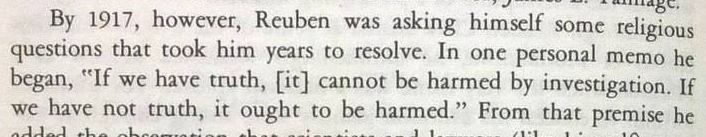
\includegraphics[width=0.4\linewidth]{articles/images/harm.png}
  \caption{J. Reuben Clark: The Church Years}
  \label{fig:clarkTruth}
\end{figure}

The quote should be cited in its full context of course. Because any and all 
sources should be found within their full context. Not only a portion. 
(See Appendix B: J. Reuben Clark: The Church Years)

Then there are the words of James E. Talmage:

\begin{displayquote}
The man who cannot listen to an argument which opposes his views either has a 
weak position or is a weak defender of it. No opinion that cannot stand 
discussion or criticism is worth holding. And it has been wisely said that the 
man who knows only half of any question is worse off than the man who knows 
nothing of it. He is not only one sided, but his partisanship soon turns him 
into an intolerant and a fanatic. In general it is true that nothing which 
cannot stand up under discussion and criticism is worth 
defending.\footnote{Editorial quoted in James E. Talmage, 
``Christianity Falsely So-Called," Improvement Era, Jan. 1920, 204.}
\end{displayquote}

George Albert Smith spoke on this very topic:

\begin{displayquote}
If a faith will not bear to be investigated; if its preachers and professors 
are afraid to have it examined, their foundation must be very 
weak.\footnote{George Albert Smith, Journal Of Discourses, v 14, page 216}
\end{displayquote}

Then M. Russell Ballard said the following counter claim:

\begin{displayquote}
We don't have to question anything in the church, don't get off into that. Just
stay in the Book of Mormon. Just stay in the Doctrine and Covenants. Just listen
to the prophets. Just listen to the apostles. We won't lead you astray, we
cannot lead you astray.\footnote{YSA Devotional, M. Russell Ballard, 2015}
\end{displayquote}

The church has released a handful of what they call Gospel Topic 
Essays.\footnote{https://www.lds.org/topics/essays?lang=eng} They are to shed
light on some of the history of the church that may or may not have been
widely known. This is a step in the right direction, however...it still feels
like the church is changing the narrative. Their history stated to the believers
has not always been the same. It has changed over time.

It is tempting to go through each of the essays...however I'm not sure I would
have the patience to go paragraph by paragraph and make notes on things found
and then look into the footnotes of each thing found.

Someday in the future I'm sure I will. There's no reason not to. If we are to
learn from the best books as it were, then the truth in those essays shouldn't
be scary. They should be welcomed with open arms. Is that possible in this day
and age of the internet? We have at our fingertips the ability to quickly search
for anything and everything. It could be considered dangerous.

I suppose, one needs to ask what is truth? If the truth can set you 
free,\footnote{John 8:32} then where exactly does the truth lay? Why is it so
difficult to find the truth at times? If the truth has been from the beginning
of the world, from before the beginning of the world, then it should be as
consistant as possible. It should be the same yesterday, today, tomorrow. All
truth should be the same and change shouldn't be a term in that narrative.

Yet the search for truth must go on.
\chapter{Revelation}

We live in a time of continuous revelation as it were. When the church was
being organized and during the time Joseph Smith was the prophet of the church,
he continued to receive revelations. The Doctrine and Covenants of the church
is full of revelations.

After Joseph's death, there doesn't appear to be many revelations coming forth
from the church. Some point to the end of polygamy, or the end of the ban 
against the blacks. There are those also who say there were other reasons
to end those things.

From a publication by David Whitmer, we find the following quote:

\begin{displayquote}
Some revelations are of God: 
some revelations are of man: 
and some revelations are of the devil.\footnote{David Whitmer, 
An Address to All Believers in Christ, in EMD 5: 198.}
\end{displayquote}

This is in regards to the failiure of the church to sell the copyright in
Canada. (See Appendix \ref{chap:believers})

Ahem, say what now? Revelations coming from the devil? As revelation? What?

How is that possible? It's been said that the devil can show himself as an 
angel, but an entire revelation from the devil? Wow, what kind of hot water
must you be in to get one of those?

Either way? How does one know if the revelation is from man, God, or the devil?
In what ways are we supposed to actually fully know that these things are
true and to do as they direct, or if we are to set them aside for they are evil?

Makes things rather complicated right?

After Joseph Smith's death, there weren't many additions to the Doctrine and
Covenants. No new revelations added. The Official Declarations 1 and 2 don't
appear to be revelations as they do not say ``Thus saith the Lord" in them,
which was known to be had in other revelations throughout the book.

So what are they exactly?

There's a revelation by Joseph F. Smith which became section 138 of the D\&C,
but nothing since then. Why is that? If we are a church that believes in
continuous revelations, why is that book not being updated? Why are there
not more revelations coming and recorded?

Time has changed things. Are people not as revelatory since the times of
Joseph Smith, Jr. when he led the church? Do we have all we need and God doesn't
see fit to speak to us in this day and age?

You might be thinking I'm being rude. But these are honest questions. I'm not
bashing the prophets who have come since Joseph Smith, Jr. I am just not aware
of actual revelations which have come along the way is all.


\appendix
\section{Appendix A: Lilith}

With all of the possible changes in the narrative throughout the years, there is
mention of a woman named Lilith. She was supposed to be Adam's first wife. But
she didn't want to follow what he said and she ran.

I include it here for a twofold purpose.

1. Do we know this isn't true for certain? It could have been removed from the
texts of the bible for all we know.

2. There is some confusion regarding Genesis 1:27 where it stats that God
created male and female. Then in the next chapter he creates them again.

Some have said there are two versions of the creation. Some have tried to state
(falsely based on the book of Moses) that this was the pre-existence creation of
Adam and Eve.

The pre existence had already been created.

The follow text is quoted from Hebrew Myths\cite{myth}:

Chapter 10: Adam's Helpmeets

(a) Having decided to give Adam a helpmeet lest he should be alone
of his kind, God put him into a deep sleep, removed one of his
ribs, formed it into a woman, and closed up the wound, Adam awoke
and said: `This being shall be named ``Woman", because she has been
taken out o f man. A man and a woman shall be one flesh.' The
title he gave her was Eve, `the Mother of 
All Living''.\footnote{Genesis II. 18-25; III. 20.}

(b) Some say that God created man and woman in His own image on
the Sixth Day, giving them charge over the 
world;\footnote{Genesis I. 26-28.} but that Eve
did not yet exist. Now, God had set Adam to name every beast, bird
and other living thing. When they passed before him in pairs, male
and female, Adam-being already like a twenty-year-old man-felt
jealous of their loves, and though he tried coupling with each
female in turn, found no satisfaction in the act. He therefore
cried: `Every creature but I has a proper matel', and prayed God
would remedy this injustice.\footnote{Gen. Rab. 17.4; B. Yebamot 632.}

(c) God then formed Lilith, the first woman, just as He had
formed Adam, except that He used filth and sediment instead of
pure dust. From Adam's union with this demoness, and with another
like her named Naamah, Tubal Cain's sister, sprang Asmodeus and
innumerable demons that still plague mankind. Many generations
later, Lilith and Naamah came to Solomon's judgement seat,
disguised as harlots of 
Jerusalem'.\footnote{Yalqut Reubeni ad. Gen. II. 21; IV. 8.}

(d) Adam and Lilith never found peace together; for when he
wished to lie with her, she took offence at the recumbent posture
he demanded. `Why must I lie beneath you?' she asked. `I also was
made from dust, and am therefore your equal.' Because Adam tried
to compel her obedience by force, Lilith, in a rage, uttered the
magic name of God, rose into the air and left him.

Adam complained to God: `I have been deserted by my helpmeet' God
at once sent the angels Senoy, Sansenoy and Semangelof to fetch
Lilith back. They found her beside the Red Sea, a region abounding
in lascivious demons, to whom she bore lilim at the rate of more
than one hundred a day. `Return to Adam without delay,' the angels
said, `or we will drown you!' Lilith asked: `How can I return to
Adam and live like an honest housewife, after my stay beside the
Red Sea?? `It will be death to refuse!' they answered. `How can I
die,' Lilith asked again, `when God has ordered me to take charge
of all newborn children: boys up to the eighth day of life, that
of circumcision; girls up to the twentieth day. None the less, if
ever I see your three names or likenesses displayed in an amulet
above a newborn child, I promise to spare it.' To this they
agreed; but God punished Lilith by making one hundred of her demon
children perish 
daily;\footnote{Alpha Beta diBen Sira, 47; Gaster, MGWJ, 29 (1880), 553 ff.}
and if she could not destroy a human
infant, because of the angelic amulet, she would spitefully turn
against her own.\footnote{Num. Rab. 16.25.}

(e) Some say that Lilith ruled as queen in Zmargad, and again in
Sheba; and was the demoness who destroyed job's 
sons.\footnote{Targum ad job 1. 15.} Yet she escaped the curse of death which 
overtook Adam, since they had parted long before the Fall. Lilith and 
Naamah not only strangle infants but also seduce dreaming men, any one of 
whom, sleeping alone, may become their 
victim.\footnote{B. Shabbat 151b; Ginzberg, LJ, V. 147-48.}

(f) Undismayed by His failure to give Adam a suitable helpmeet,
God tried again, and let him watch while he built up a woman's
anatomy: using bones, tissues, muscles, blood and glandular
secretions, then covering the whole with skin and adding tufts of
hair in places. The sight caused Adam such disgust that even when
this woman, the First Eve, stood there in her full beauty, he felt
an invincible repugnance. God knew that He had failed once more,
and took the First Eve away. Where she went, nobody knows for
certain.\footnote{Gen. Rab. 158, 163-64; Mid. Abkir 133, 135; 
Abot diR. Nathan 24; B. Sanhedrin 39a.}

(g) God tried a third time, and acted more circumspectly. Having
taken a rib from Adam's side in his sleep, He formed it into a
woman; then plaited her hair and adorned her, like a bride, with
twenty-four pieces of jewellery, before waking him. Adam was
entranced.\footnote{Gen. II. 21-22; Gen. Rab. 161.}

(h) Some say that God created Eve not from Adam's rib, but from a
tail ending in a sting which had been part of his body. God cut
this off, and the stump-now a useless coccyx-is still carried by
Adam's descendants.\footnote{Gen. Rab. 134; B. Erubin 18a.}

(i) Others say that God's original thought had been to create two
human beings, male and female; but instead He designed a single
one with a male face looking forward, and a female face looking
back. Again He changed His mind, removed Adam's backward-looking
face, and built a woman's body for it.\footnote{B. Erubin 18a.}

 (j) Still others hold that Adam was originally created as an
androgyne of male and female bodies joined back to back. Since
this posture made locomotion difficult, and conversation awkward,
God divided the androgyne and gave each half a new rear. These
separate beings He placed in Eden, forbidding them to 
couple.\footnote{Gen. Rab. 55; Lev. Rab. 14.1: Abot diR. Nathan 1.8; B.
Berakhot 61a; B. Erubin 18a; Tanhuma Tazri'a 1; Yalchut Gen. 20;
Tanh. Buber iii.33; Mid. Tehillim 139, 529.}

There is no way of knowing if these thoughts are true or if they are of fable.
The truth will eventually come forth in time naturally, but with all of the
changes of the Bible that have taken place, who is to know for sure exactly if
what is in the Bible can be taken as truth.

Either way, this is an interesting insight into human thought on the matter.
Changes come and go, there will always be changes it would seem.
\chapter{J. Reuben Clark: The Church Years}

By 1917, however, Reuben was asking himself some religious questions that took 
him years to resolve. In one personal memo he began, ``If we have truth, [it] 
cannot be harmed by investigation. If we have not truth, it ought to be harmed." 
From that premise he added the observation that scientists and lawyers 
(like himself) were not blindly believing and that they must refuse to be 
deceived by others or by their own wishful thinking. ``A lawyer must get at 
facts, he must consider motives -- he must tear off the mask and lay bare the 
countenance, however hideous. The frightful skeleton of truth must always be 
exposed ... [the lawyer] must make every conclusion pass the fiery ordeal of 
pitiless reason. If their conclusions cannot stand this test, they are false." 
During the same year the increasingly introspective lawyer asked himself the 
questions: Are we not only entitled, but expected to think for ourselves? 
Otherwise where does our free agency come in? His answer was a resounding: 
``If we are blindly to follow some one else we are not free agents.... 
That we may as a Church determine for ourselves our course of action, is 
shown by the Manifesto [abandoning the practice of polygamy]. We may not 
probably take an affirmative stand, i.e., adopt something new but we may 
dispense with something." Perhaps he had never before questioned the assumptions 
that lay behind some of the simple faith of his youth, but at midlife J. 
Reuben Clark, Jr. proclaimed that there must be no forbidden questions in 
Mormonism.

The directions to which his philosophy of religious inquiry led him were 
indicated in his musings about two essentials of Mormonism: the revelations of 
Joseph Smith, Jr. and the Church belief in progression toward godhood. As he 
examined the revelations in the Doctrine and Covenants concerning the structure 
of the Church government, Reuben Clark wondered to what extent Joseph Smith's 
reading or experience, ``his own consciousness," had contributed to what he set 
down, and when Reuben pondered the Mormon belief in the potential of individuals 
to attain the godly stature of their Father in Heaven, his logical mind boggled 
a bit. ``Is Space or occupied portions of it divided among various deities -- 
have they great `spheres of influence'? War of Gods -- think of wreck of matter 
involved -- if matter used -- or would it be a war of forces?" In his 
mid-forties, he regarded these as legitimate doctrinal inquiries but soon 
realized that each question concerning doctrine led to other questions, each 
of which was further removed from rational verification. Reuben soon came to the 
conclusion he described in later years to the non-Mormon president of George 
Washington University: ``For my own part I early came to recognize that for me 
personally I must either quit rationalizing ... or I must follow the line of 
my own thinking which would lead me I know not where."

But J. Reuben Clark soon recognized where an uncompromising commitment to 
rational theology would lead him, and he shrank from the abyss. 
``I came early to appreciate that I could not rationalize a religion for myself, 
and that to attempt to do so would destroy my faith in God," 
he later wrote to his non-Mormon friend. ``I have always rather worshipped 
facts," he continues,``and while I thought and read for a while, many of the 
incidents of life, experiences and circumstances led, unaided by the spirit of 
faith, to the position of the atheist, yet the faith of my fathers led me to 
abandon all that and to refrain from following it.... For me there seemed to be 
no alternative. I could only build up a doubt. --If I were to attempt to 
rationalize about my life here, and the life too come, I would be drowned in 
a sea of doubt."

All the confidence of J. Reuben Clark's commitment to rational inquiry in 
religious matters evaporated. He had once believed that in intellectual faith 
``we may not probably take an affirmative stand, i.e., adopt something new but 
we may dispense with something," but Reuben found that such an attempt could 
only lead to dispensing with everyting [sic]. As he cast about for some way of 
explaining his position to others, he discovered an anecdote about Abraham 
Lincoln, who justified reading the Bible despite his reputed agnosticism with 
the comment: ``I have learned to read the Bible. I believe all I can and take 
the rest on faith." To a friend, Reuben related the Lincoln story and added, 
``Substituting in the substance the words `our Mormon Scriptures,' you will 
have about my situation." He later commended that anecdote to a general 
conference of the Church. Convinced that no religious faith could withstand 
uncompromising intellectual inquiry, Reuben concluded that in Babylon as well 
as in Zion, the refusal to rationalize one's religious beliefs was the highest 
manifestation of faith.

\cite{clark}
\chapter{An Address to All Believers in Christ}

Joseph looked into the hat in which he placed the stone, and received a 
revelation that some of the brethren should go to Toronto, Canada, and that 
they would sell the copyright of the Book of Mormon. Hiram Page and Oliver 
Cowdery went to Toronto on this mission, but they failed entirely to sell the 
copyright, returning without any money. Joseph was at my father's house when 
they returned. I was there also, and am an eye witness to these facts. Jacob 
Whitmer and John Whitmer were also present when Hiram Page and Oliver Cowdery 
returned from Canada. Well, we were all in great trouble; and we asked Joseph 
how it was that he had received a revelation from the Lord for some brethren to 
go to Toronto and sell the copyright, and the brethren had utterly failed in 
their undertaking. Joseph did not know how it was, so he enquired of the Lord 
about it, and behold the following revelation came through the stone: 
`Some revelations are of God: some revelations are of men: and some 
revelations are of the devil.' So we see that the revelation to go to 
Toronto and sell the copyright was not of God, but was of the devil 
or of the heart of man.

\cite{whitmer}

\backmatter
\printbibliography
\thispagestyle{empty}

\end{document}